\documentclass[rmp,10pt,onecolumn,fleqn,notitlepage]{revtex4-1}

\usepackage{graphicx}
\usepackage{wrapfig}
\usepackage{color}
\usepackage{latexsym,amsmath}
\usepackage{physics}
\usepackage{chemformula}
\usepackage{tabularx}
\usepackage{float}
\usepackage{siunitx}
\usepackage{amssymb}
\usepackage[caption=false, justification=right]{subfig} % sfancula la formattazione delle figure se caption è messo su true
\usepackage{multirow}

% Listing packages
\usepackage{xcolor}
\usepackage{listings}
\usepackage{framed}
\usepackage{inconsolata} % To change the listing font

%------------------------------------------------------------------------
% URL package and setting
%------------------------------------------------------------------------
\definecolor{linkcolor}{rgb}{0,0,0.65} %hyperlink
\definecolor{linescolor}{rgb}{0.65,0.16,0.16}
\definecolor{cool}{RGB}{49,54,149}
\definecolor{hot}{RGB}{165,0,38}
\usepackage[pdftex,colorlinks=true, pdfstartview=FitV, linkcolor= linescolor, citecolor= linescolor, urlcolor= linkcolor, hyperindex=true,hyperfigures=true]{hyperref} %hyperlink%

\usepackage{fancyhdr} % To change page setting

%------------------------------------------------------------------------
% PAGE SETTING
%------------------------------------------------------------------------
\pagestyle{fancyplain}
\fancyhf{}
\fancyfoot[R]{\textbf{\thepage}}
\fancyfoot[L]{Università degli Studi di Padova - Dipartimento di Fisica e Astronomia Gailelo Galilei} 
%\fancyhead[L]{\textbf{Advanced Physics Laboratory Report}}
\fancyhead[L]{\ifnum\value{section}>0\nouppercase{\textbf{\leftmark}\fi}}
\fancyhead[R]{\textbf{Alice Pagano - Francesca Dodici}}
\renewcommand{\headrulewidth}{0.2pt}
\renewcommand{\footrulewidth}{0.1pt}


% Section style


%\renewcommand{\thesection}{\textbf{\arabic{section}}}
%\renewcommand{\thesubsection}{\thesection.\textbf{\arabic{subsection}}}
%\renewcommand{\thesubsubsection}{\textbf{\thesection.\arabic{subsection}.\arabic{subsubsection}}}


\renewcommand{\thesection}{\textbf{\Roman{section}}}
\renewcommand{\thesubsection}{\textbf{\arabic{subsection}}}
\renewcommand{\thesubsubsection}{\textbf{\Alph{subsubsection}}}


%Redefine \thesubsection as \thesection.\alph{subsection}. (\alph replaces the default \arabic; you could also choose, e.g., \Alph, \roman, and \Roman.)





% Figure style
\renewcommand{\tablename}{\textbf{TAB.}}
\renewcommand{\thetable}{\textbf{\arabic{table}}}

\renewcommand{\figurename}{\textbf{FIG.}}
\renewcommand{\thefigure}{\textbf{\arabic{figure}}}

%------------------------------------------------------------------------
% BIBLIOGRAPHY FILE AND SETTING
%------------------------------------------------------------------------
\bibliographystyle{aipnum4-1}
\setcitestyle{numbers,square}

% Intendation
\setlength\parindent{9pt}


\begin{document}

% Set figure caption in bold
\captionsetup[figure]{labelfont={bf},labelformat={default},labelsep=period,name={FIG.}}

%------------------------------------------------------------------------
%	IMMAGINI FRONTESPIZIO
%------------------------------------------------------------------------
\begin{figure}[H]
\begin{minipage}{0.25\linewidth}

\includegraphics[width=\linewidth]{logo_DFA.jpg}
\end{minipage}
\hfill
\begin{minipage}{0.35\linewidth}

\includegraphics[width=\textwidth]{logo_800anni.png}
\end{minipage}
\end{figure}
% LINEE
\noindent\makebox[\linewidth]{\color{linescolor} \rule{0.85\paperwidth}{1.2 pt}}
\noindent\makebox[\linewidth]{\color{linescolor} \rule[0.3cm]{0.85\paperwidth}{1pt}}

\title{Measurement of the critical temperature of a superconductor via resistance measurements}
\author{Alice Pagano - 1236916 - alice.pagano@studenti.unipd.it \\ Francesca Dodici - 1237602 - francesca.dodici@studenti.unipd.it}
\date{\today}

\begin{abstract}

Superconductivity is a phenomenon occurring in certain materials that display exactly zero electrical resistance and expulsion of magnetic fields  when cooled below a characteristic critical temperature $T_c$. It is a macroscopic quantum phenomenon whose
special physical properties have attracted the attention of many physicists and electric engineers since its discovery by Onnes in 1911. 
In this Report, we discuss the realization of an experimental apparatus for the estimation of the critical temperature of an unknown ceramic cuprate superconductor sample by measuring the drop in electrical resistance.
\end{abstract}

\maketitle


\noindent\makebox[\linewidth]{\color{linescolor} \rule[0.1cm]{0.85\paperwidth}{1pt}}

%------------------------------------------------------------------------
%INDICE
%------------------------------------------------------------------------
{
  \hypersetup{linkcolor=black}
  \tableofcontents
}
\noindent\makebox[\linewidth]{\color{linescolor} \rule[-0.2cm]{0.85\paperwidth}{1pt}}
\noindent\makebox[\linewidth]{\color{linescolor} \rule[0.3cm]{0.85\paperwidth}{1.2 pt}}
\pagebreak
%------------------------------------------------------------------------
%TESTOH
%------------------------------------------------------------------------
% Start counting page after the first one which is the title
\pagenumbering{gobble} 
\newpage
\pagenumbering{arabic}

\section{Introduction}
\label{sec:introduction}

In normal conductors, the flow of an electrical current is subject to some resistance to the motion of electrons through the material. A difference of potential must be constantly applied to keep the current going and replace the energy dissipated by the resistance \cite{sheahen1994introduction}. 

Superconductivity is the phenomenon for which a material, below a certain critical temperature $T_c$, undergoes a phase transition that causes its electrical resistivity to suddenly drop to zero. Having no resistance, a supeconductor is able to carry a current indefinitely without having to apply a potential difference across it. This phenomenon was observed for the first time by Kamerlingh Onnes in Leiden in 1911, three years after he first liquified helium \cite{kittel_2004}. 

The absence of electrical resistance below $T_c$ is not the only peculiar feature of superconductors: they also display the so called Meissner effect in which they behave as perfect diamagnets provided that the applied magnetic field is not too strong.

The first metal discovered to display superconductivity was mercury, with a $T_c$ of \SI{4.1}{\kelvin}  \cite{onnes1911disappearance}. In the subsequent 50 years, many other metals were found to have superconductive behaviour at these very low temperatures. By the 1960s, certain alloys of niobium were also found to have a superconductive transition with a $T_c$ higher than that of pure metals, but still in the liquid helium range. 

Since the discovery of superconductivity many scientists tried to establish a theoretical explanation of the phenomenon. As a result in 1957, Bardeen, Cooper, and Schrieffer developed the so called BCS theory. In this theory, they ascribed superconductivity to an attractive interaction between two electrons through electron–phonon interaction. To put it simply, they assumed that when one electron interacts with a positive ion in the lattice, it deforms the latter so that then, a second electron of compatible momentum can interact with the ion in the distorted lattice so as to minimize the energy. The interacting electrons are said to form a pair called Cooper pair. The electrons of a pair have equal and opposite momentum; one in spin up state and the other in spin down state, so that the total spin of a pair is zero \cite{BCSth}.

In 1986 the observation of superconductivity at temperatures up to \SI{38}{\kelvin} in lanthanum copper oxides doped with barium or strontium  \cite{bednorz1986possible} paved the way to high temperature superconductivity. Since then, several other ceramics, based on copper oxide, were found to remain superconductive even at temperatures beyond \SI{100}{\kelvin}, which is high enough to allow liquid nitrogen based cooling (as the boiling temperature of \ch{N} is \SI{77}{\kelvin}). 
Examples of these materials displaying high temperature superconductivity are yttrium barium copper oxide or YBCO with $T_c$ up to \SI{92}{\kelvin} and bismuth strontium calcium copper oxide or BSCCO which can reach $T_c$ up to \SI{110}{\kelvin}. 

As of today, high temperature superconductivity remains one of the biggest unsolved problems in theoretical condensed matter physics. In fact, these cuprate superconductors differ from conventional ones not only in their high values of $T_c$, but also in a set of physical properties that cannot be described by the classical Bardeen–Cooper–Schrieffer (BCS) scheme.
In fact, these materials are generally very complex, multi-layered crystals, making theoretical modelling difficult. In these complicated substances, several phase transitions (structural, magnetic, superconductor, etc.) occur, and mixed states are allowed \cite{cuprate_review}. Because of this, the same compound can be found in different phases, each with a different $T_c$. Moreover, the transition to the superconducting state is usually less sharp than in metallic low $T_c$ superconductors \cite{HTC_springer}, leading to ambiguities in the estimation of $T_c$. For these reasons, the values of $T_c$ reported in literature might be a bit different depending on whether $T_c$ is considered as the temperature at which the resistivity becomes exactly zero or as centroid of the transition region. 

The aim of this Report, is to estimate the critical temperature of a small bar of either YBCO or BSCCO. Based on our results, we will infer the nature of the sample considered.
In TAB. \ref{tab:theoretical_tc} are reported the critical temperatures associated to the most common phases of these materials.

\vspace{1cm}

\begin{table}[h!]
\centering
    \sisetup{separate-uncertainty}
    \begin{tabular*}{0.5\linewidth}{@{\extracolsep{\fill}}
    c%S[table-format=3.1(1)] 
    c%S[table-format=3.1(1)]
    c%S[table-format=3.1(1)]
    }
        \toprule
     \textbf{YBCO} & \textbf{BSCCO-2212} & \textbf{BSCCO-2223}  \\
        \colrule
     \SI{90}{\kelvin} & \SI{85}{\kelvin} & \SI{110}{\kelvin}  \\
    \botrule
    \end{tabular*}
    \caption{Theoretical critical temperatures for YBCO or \ch{YBa2Cu3O7}, BSCCO-2212 or \ch{Bi2Sr2Ca1Cu2O_{8+y}} and  BSCCO-2223 or \ch{Bi2Sr2Ca2Cu3O_{10+y}}. Here $T_c$ is taken as temperature at which the resistivity becomes exactly zero \cite{cuprate_review}. }
    \label{tab:theoretical_tc}
\end{table}


\clearpage 

\section{Experimental setup}
\label{sec:experimental_setup}

In this section we describe the experimental setup engineered for the measurements of the critical temperature of the sample. A schematic depiction is provided in FIG. \ref{fig:setup}.

The core of the apparatus is the \textit{vacuum chamber} of the cryostat in which the sample and the diagnostics are located. The pressure inside the chamber is monitored using a Pirani gauge and the temperature of the system is lowered using a \textit{cryocooler}. The cryocooler has a first stage reaching \SI{70}{\kelvin} and a \textit{cold finger} reaching up to \SI{20}{\kelvin}. A \textit{radiation shield} is anchored on the first stage, whereas the sample holder is located on top of the cold finger.
It is essential to lower the pressure to about $10^{-2} \divisionsymbol 10^{-3}$\si{\milli \bar} in order to reduce the thermal coupling of the sample with the external environment and improve the cooling speed. To this end, a \textit{rotatory pump} is employed.

Moreover, to monitor the temperature of the system, two different platinum thermometer Pt100 are used. The first one is mounted on the cold finger and connected to an Arduino to provide automatic temperature measurements. 
From now on, we shall refer to it as \textit{Pt100-cf} for the sake of simplicity. The second one, \textit{Pt100-s}, is located in close proximity to the sample, thus providing a more accurate estimate of the temperature of the sample itself. It is connected to a \textit{temperature bridge} circuit, described in detail in SEC. \ref{subsec:thermometer_bridge}.
Furthermore, the sample is connected to an \textit{amplifier circuit}, which is essential for measuring the voltage drop at the critical temperature since the electrical resistance of the ceramic sample is expected to be extremely small.
Both the amplifier circuit and the temperature bridge are soldered on a NIM module.

Additionally, on one side of the sample holder, there is also a \textit{heater}. This consists of a simple \SI{50}{\ohm} resistance powered though a DC power supply. It is utilized to control the temperature of the sample. As a matter of fact, by balancing the power dissipated on the heater through Joule effect with the cooling power of the cryocooler, one is able to fix the temperature of the sample around a desired value.

The \textit{sample} is located inside a small aluminum box and wrapped in a thin layer of mylar to isolate it electrically from the rest of the chamber without undermining its thermal coupling with the cold finger.

The sample and the thermometers are connected to their respective circuits using \textit{resistive wires} to reduce the thermal coupling with the outside of the chamber. Ordinary conductive (although very thin) wires are utilized only to power the heater. 

\begin{figure}[h!]
    \centering
    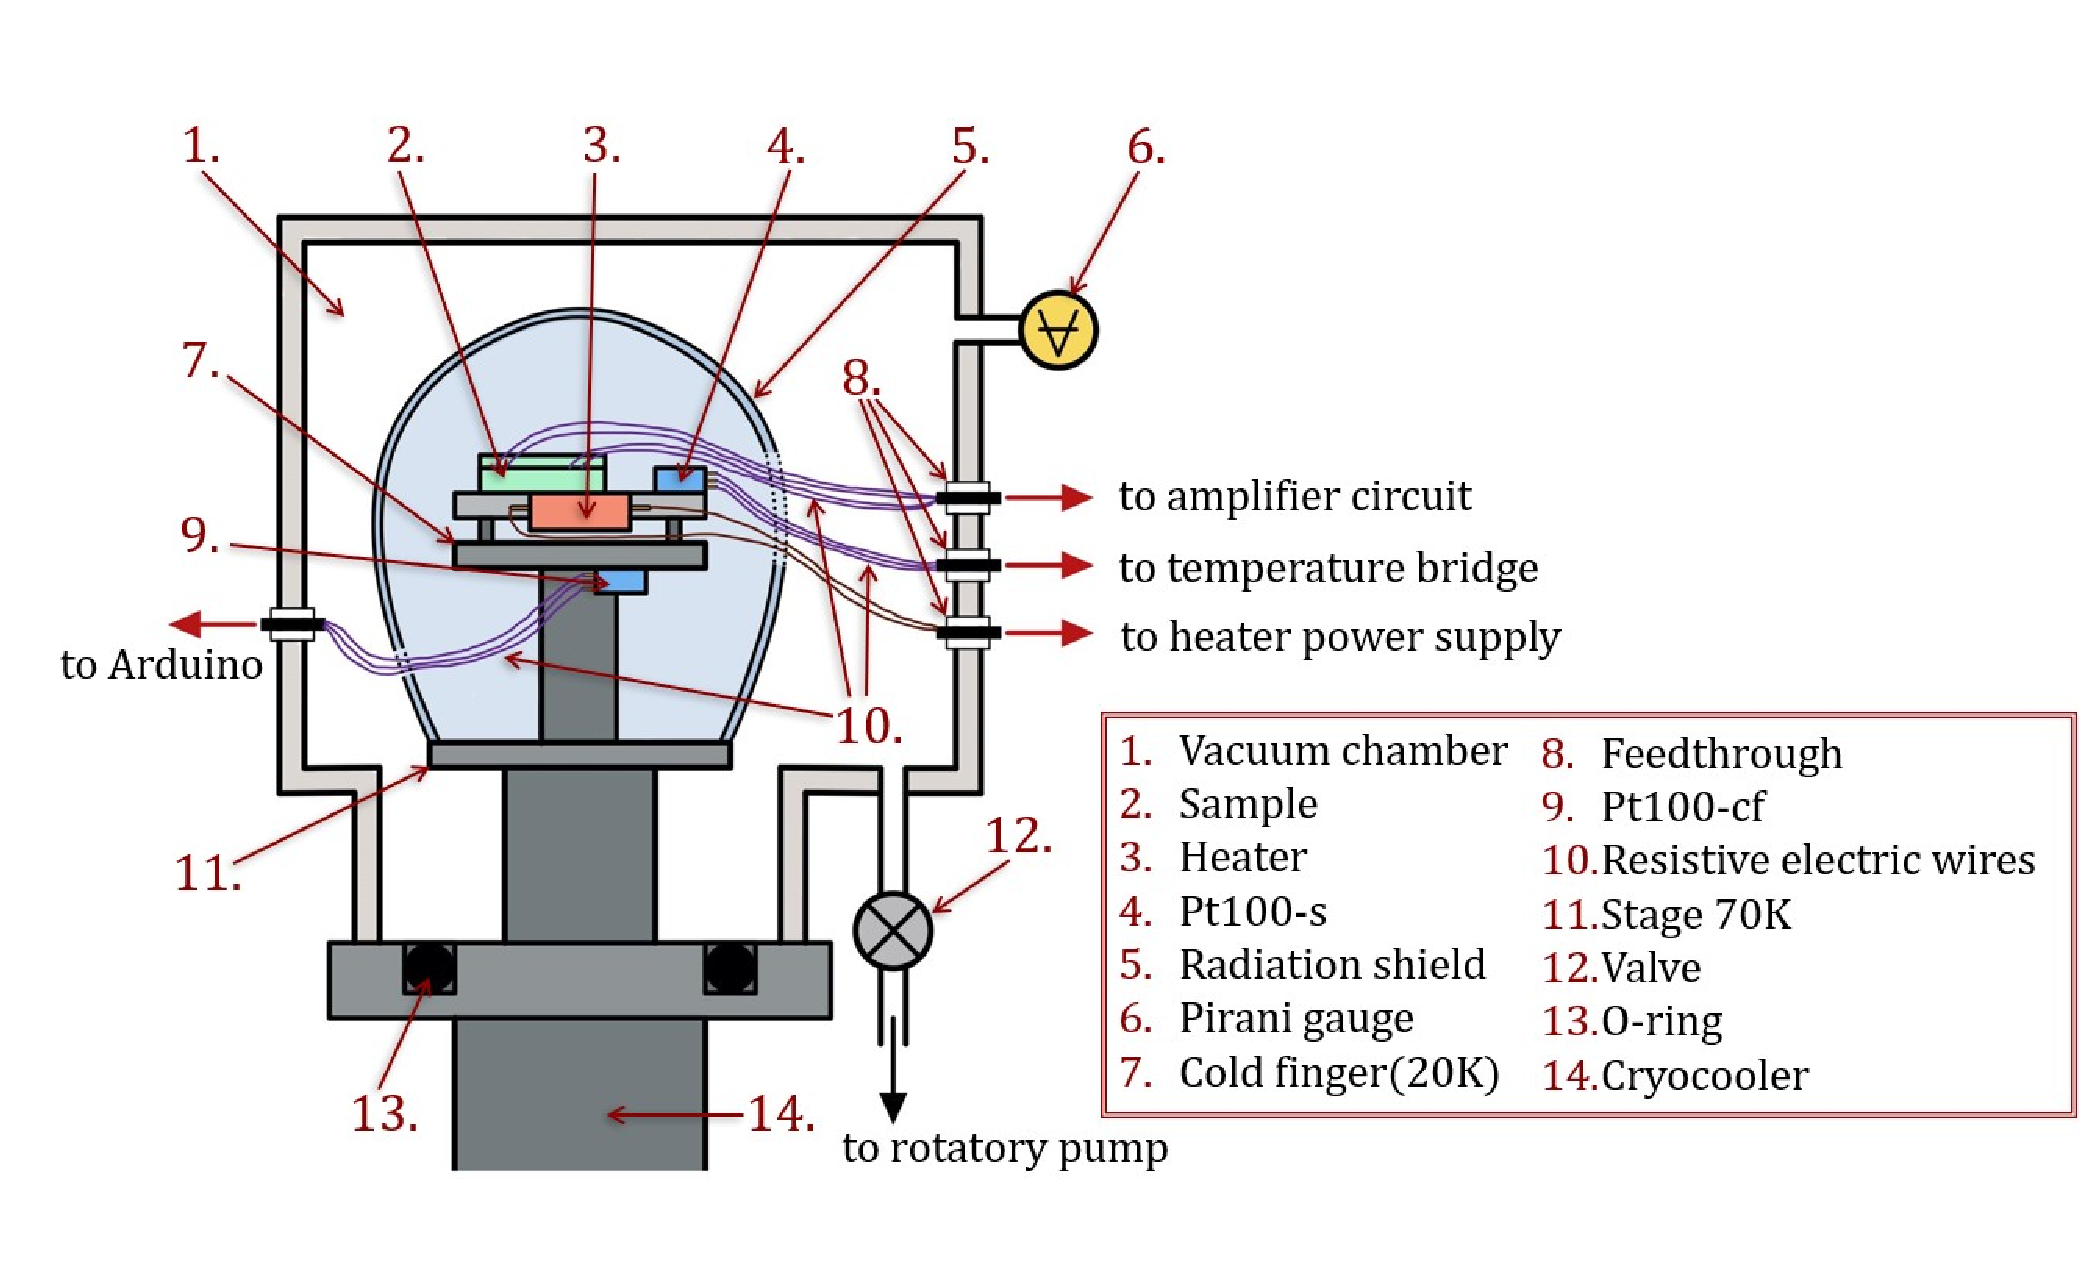
\includegraphics[width=\textwidth]{image/schemes/Setupscheme.pdf}
    \caption{Scheme of the experimental setup inside the cryostat and its components.}
    \label{fig:setup}
\end{figure}


\subsection{Thermometer bridge}
\label{subsec:thermometer_bridge}

As previously anticipated in SEC. \ref{sec:experimental_setup}, the most accurate estimation of the sample's actual temperature is obtained using the Pt100-s connected to the three-wire Wheatstone bridge outlined in FIG. \ref{fig:T_circ}.

A Pt100 thermometer exploits the linear relationship between the electrical resistivity of a metal and its temperature according to the following equation:
\begin{equation}
    \rho(T) = \rho_0(1 + \alpha T)
\label{eq:ResTPt100}
\end{equation}
where $\rho_0$ is the residual resistivity for low $T$ and $\alpha$ is the temperature coefficient ($4 \cdot 10^{-3}$ \si{\per \kelvin}). Thus, by measuring the resistance $R(T)$ of the thermometer, it is possible to estimate the corresponding temperature using designated calibration tables.

The circuit is powered by an AC generator  providing an alternate signal with \SI{30}{\hertz} frequency and amplitude set to $V_g = 6.2\, \makebox{Vpp}$. The generator is equipped with an insulation transformer (i.e. with a 1:1 transforming ratio) to prevent accidental shorting of $R_v$ with the ground.

\begin{figure}[H]
    \fontsize{10pt}{12pt}\selectfont
    \begin{minipage}{0.42\linewidth}\setlength{\parindent}{9pt}
    In the scheme, $R_{T}$ denotes the resistance of Pt100-s, which is \SI{100}{\ohm} at \SI{0}{\celsius} and, as said, decreases linearly with temperature.
    
     $R_1$ and $R_2$ have resistances of $(11.98\pm0.06)\, \si{\kilo\ohm}$  and $(12.00\pm0.06)\, \si{\kilo\ohm}$  respectively and are specifically selected to be as similar as possible. Moreover, their value is chosen to be high enough to reduce the power dissipated on $R_T$, preventing self-heating. 
     
     The variable resistor $R_v$ is a helipot with a full-scale of \SI{100}{\ohm} and 50 divisions per revolution (i.e. the smallest division is \SI{0.2}{\ohm}). 
    
    Finally, the small resistors denoted with $r$ represent the resistances of the three wires connecting Pt100-s to the circuit outside.
    \end{minipage}
\hfill
    \begin{minipage}{0.5\linewidth}
    \centering
    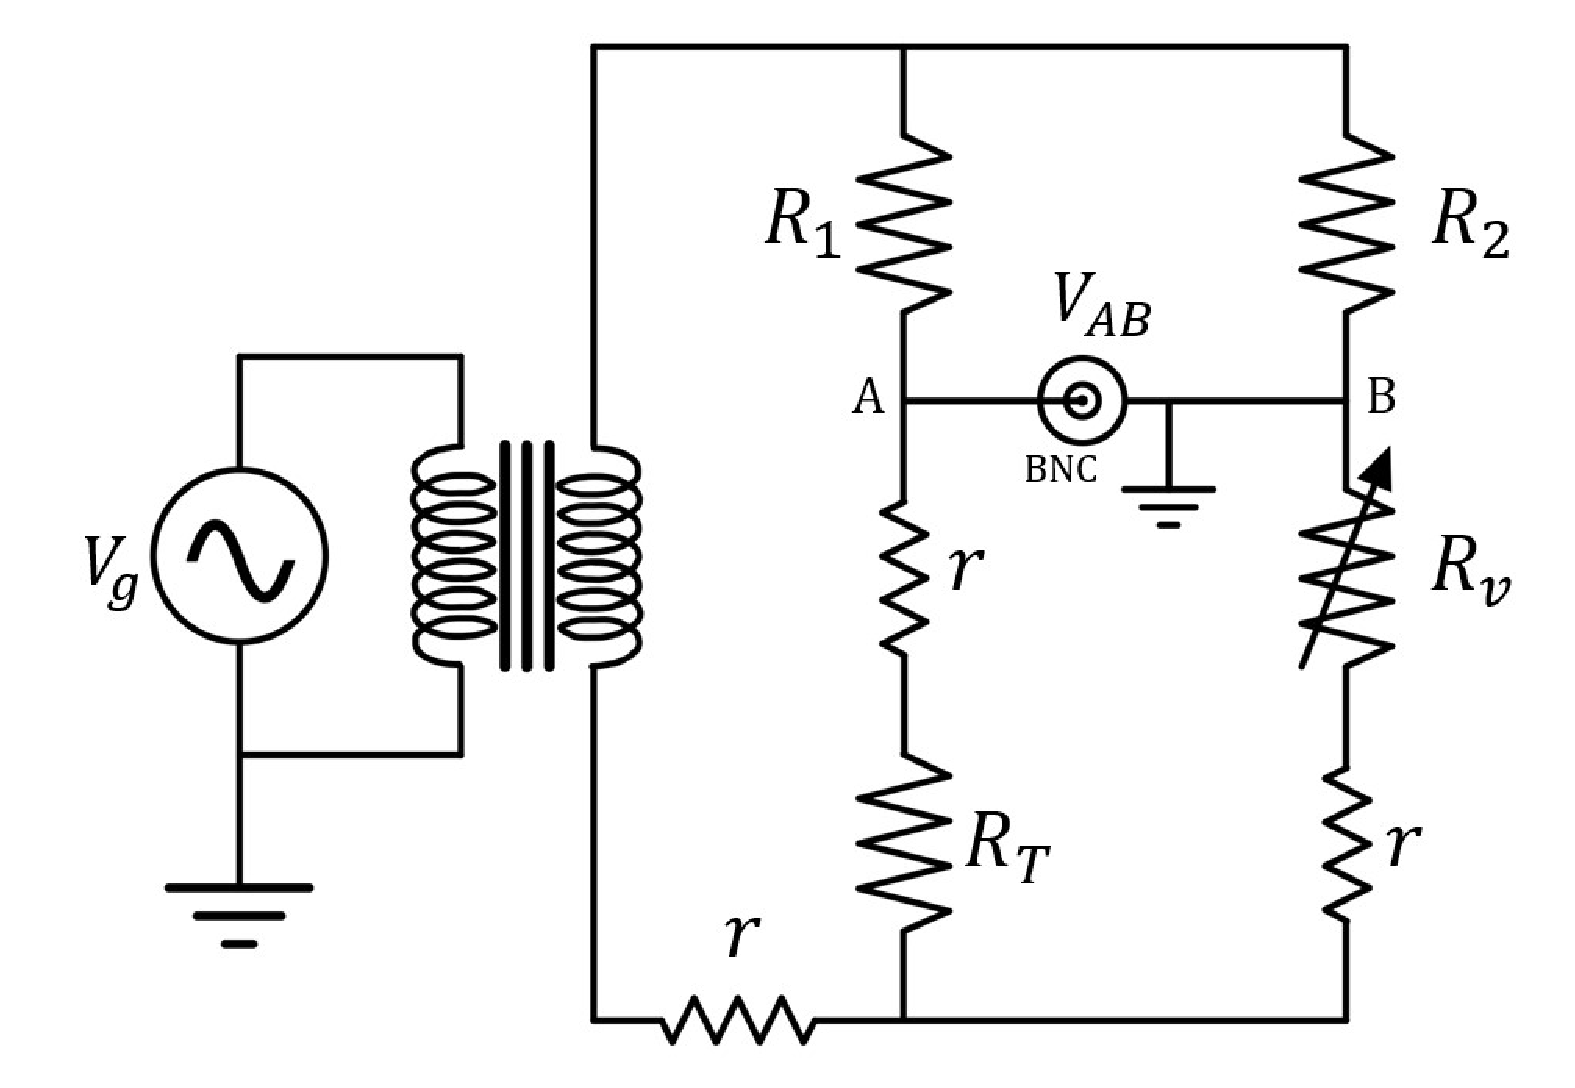
\includegraphics[width=0.85\textwidth]{image/schemes/Term_circ.pdf}
    \caption{Scheme of the three-wire bridge circuit connected to the Pt100-s on the sample holder.}
    \label{fig:T_circ}
    \end{minipage}
\end{figure}

The circuit is designed in a way such that the output voltage $V_{AB}$ should be zero when
    \begin{equation}
        R_{T}=\frac{R_{2}}{R_{1}}R_{v}
    \label{eq:Rt}
    \end{equation}
Since $R_1 \approx R_2$, this condition is approximately satisfied when $R_v = R_T$. This way, by setting $R_v$ to a value for which $V_{AB} = 0$, we can infer the resistance of the thermometer $R_T$. 

To amplify the differential voltage $V_{AB}$ in output and exploit the full sensitivity of the helipot for the reading, $V_{AB}$ is sent to a \textit{lock-in amplifier}.

Notice that the resistances $r$ of the wires do not appear in the condition of balance. In fact, although their resistances are not negligible ($r \sim $\SI{10}{\ohm}), with this design, since the wires have the same length and are of the same type, they have no effect on the condition of balance. 

It can be easily verified that, with the chosen components, the power dissipated on $R_T$ is small enough to avoid self-heating which would disrupt the coupling between sample and thermometer. As a matter of fact, at \SI{0}{\celsius} when $R_T=$\SI{100}{\ohm}: 
\begin{subequations}
\begin{align}
   V_B & = V_g \frac{R_T}{R_T+R_2} \approx 50 \, \si{\milli\volt}\\
    P_T & = \frac{V_{B}^{2}}{R_{T}} \approx 2.5 \cdot 10^{-5} \, \si{\watt}
\end{align}
\end{subequations}
which is quite reasonable. Moreover, as $T$ decreases, so does $R_T$, further improving this result.

\pagebreak

\subsection{Amplifier circuit}
\label{subsec:amplifier_circuit}
To detect at which temperature the drop in electrical resistivity of the superconductor sample occurs, a constant DC current is driven through it and the voltage drop $V_{SC}$ across it should be taken as output signal. However, the electrical resistance of the ceramic sample $R_{SC}$ is expected to be extremely small, with order of magnitude comparable to that of contact resistances. For this reason, in order to be able to measure the resistance drop at $T_c$, $V_{SC}$ must be amplified. To achieve this, a differential amplifier INA114 is employed. 
The scheme of the amplifier circuit is provided in FIG. \ref{fig:A_circ}.

\begin{figure}[H]
      \fontsize{10pt}{12pt}\selectfont
    \begin{minipage}{0.42\linewidth}\setlength{\parindent}{9pt}
    The INA114 is a 8-pin differential amplifier whose gain can be set to any value from 1 to 10,000. This is achieved simply by choosing an appropriate value for the external gain resistor $R_G$ according to the following formula:
    \begin{equation}
        G = 1 + \frac{50\, \si{\kilo \ohm}}{R_G}
    \end{equation}
    When setting the gain, one must be careful to choose a value high enough as to provide a good amplification of $V_{SC}$ but not too high, as it will cause oscillations in the output signal $V_{out}$. In this case, we choose to set the gain to $G \sim 500$. To this purpose we use a resistor $R_G = (98.5 \pm 0.5)\, \si{\ohm}$ resulting in $G = 509 \pm 3$. 
    The INA114 is driven by a dual power supply with $\pm \SI{12}{\volt}$ provided by the NIM rack. 
    To reduce the high frequency noise, two decoupling capacitors $C = 1 \, \si{\micro \farad}$ are inserted close to the pins as shown in FIG. \ref{fig:A_circ}. 
    \end{minipage}
\hfill
    \begin{minipage}{0.5\linewidth}
    \centering
    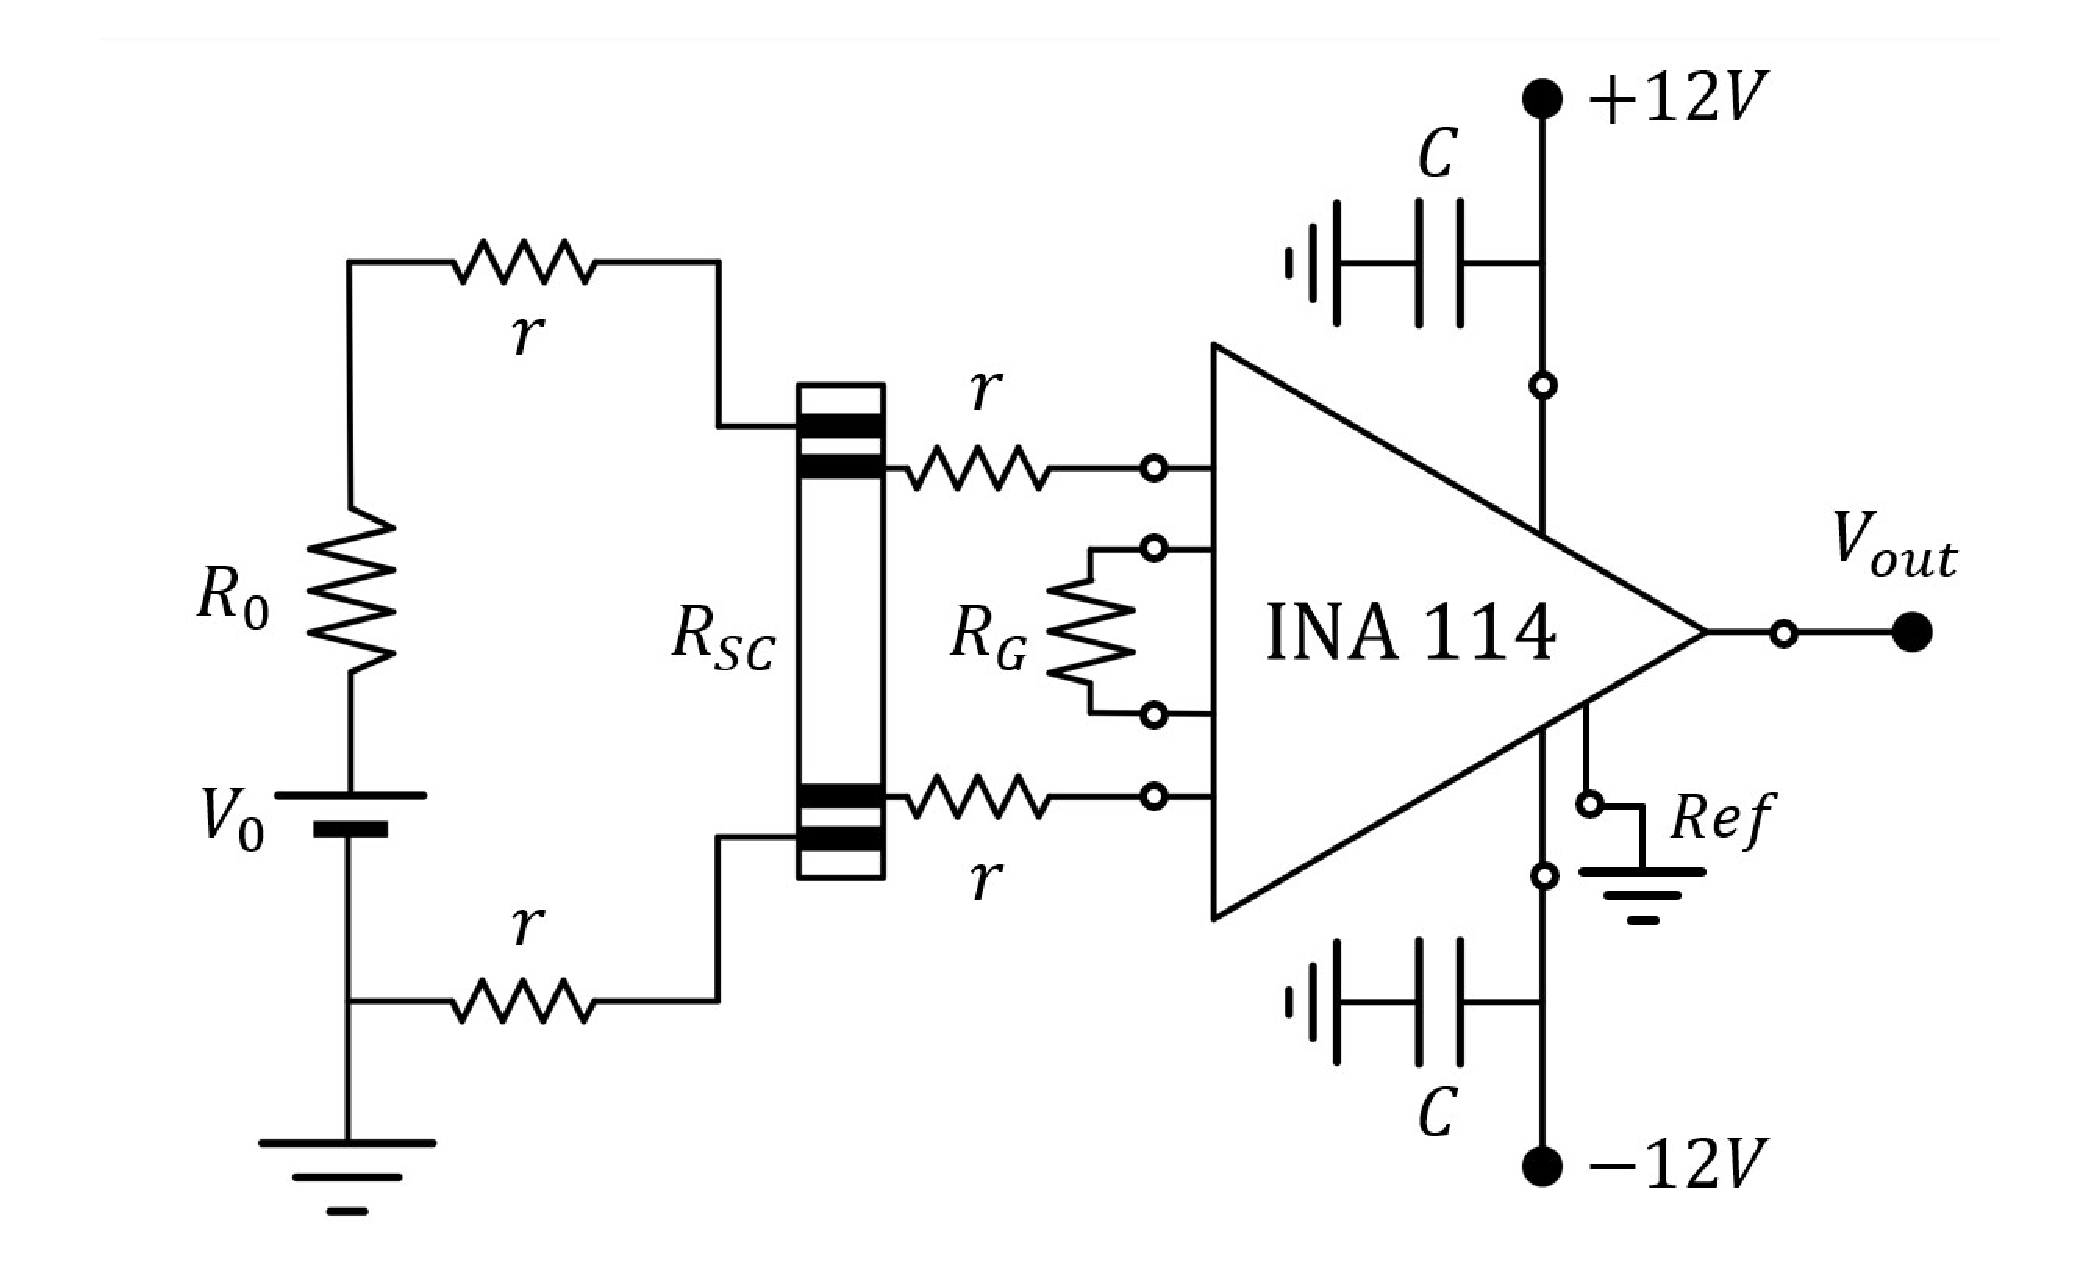
\includegraphics[width=\textwidth]{image/schemes/Amp_circ_v2.pdf}
    \caption{Scheme of the differential amplifier circuit connected to the sample. The small resistances $r$ represent the resistive wires inside the cryostat.}
    \label{fig:A_circ}
    \end{minipage}
\end{figure}

As in the previous scheme for the three-wire bridge, the small resistances $r$ represent the four wires connecting the sample to the outside of the chamber, but have no net effect on the response of the circuit.

Additionally, to have an approximately constant current flowing through the sample, in spite of the variations in the value of $R_{SC}$ with the temperature, the input resistance $R_0$ is added to create a voltage divider such that, if $R_0 \gg R_{SC}$, we can approximate:
\begin{equation}
    V_{SC}=V_0\frac{R_{SC}}{R_{SC}+R_0}\approx R_{SC}\frac{V_0}{R_0}=R_{SC}I
\label{eq:I_const}
\end{equation}
Thus, having a constant $I$, the direct proportionality between $R_{SC}$ and $V_{SC}$ can be exploited to derive the sample's resistance from the output tension, with $I = (6.03 \pm 0.03)\, \si{\milli \ampere}$.

It is possible to estimate the value of $R_{SC}$ by measuring $V_{out}$ and inverting EQ. (\ref{eq:I_const}):
\begin{equation}
    R_{SC} = \frac{V_{SC}}{I} = \frac{V_{out}}{G} \cdot \frac{R_0}{V_0}
    \label{eq:R_SC_estimate}
\end{equation}
At room temperature, with $V_0 = (6.000 \pm 0.005)\, \si{\volt}$ the output of the circuit is $V_{out} = (64.3 \pm 0.1)\, \si{\milli \volt}$ with error by propagation of random errors. Consequently, we estimate $R_{SC}=(0.020 \pm 0.002)\,\si{\ohm}$ at room temperature. In light of this, since $R_{SC}$ is very small, by choosing $R_0 =(0.995 \pm 0.005)\, \si{\kilo \ohm}$, the approximation of having constant current in the generator loop is verified with a relative error in the estimate of $V_{SC}$ using EQ. (\ref{eq:I_const}) of the 0.001\%.  

The final precaution that must be taken when choosing the components of the circuit is that the power dissipated on the sample $P_{SC}$ must be as small as possible to prevent overheating by Joule effect, which will increase cooling times and worsen the coupling with the Pt100-s.
In this case, with $R_{SC} = 0.01$\si{\ohm}, and constant current we have a dissipated power of the order of:
\begin{equation}
    P_{SC}=R_{SC} I^2\approx 3.6\cdot 10^{-7}\, \si{\watt}
\end{equation}
which is low enough and is expected to become even smaller with the decrease of $R_{SC}$ at lower temperatures in compliance with EQ. (\ref{eq:ResTPt100}).

\clearpage


\section{Data acquisition procedure}
\label{sec:data_acquistion_procedure}

After having assembled the experimental setup as described in the previous sections, it is finally possible to begin collecting data. To this purpose, the following procedure is followed. 

Firstly, the rotatory pump is activated to lower the pressure inside the chamber. Once the desired level of vacuum is achieved ($\sim 10^{-3}$ \si{\milli \bar}) the cryocooler is turned on and the cooling procedure is initiated. 

The DC voltage of the amplifier circuit is set to $V_0=\SI{6}{\V}$. Since below $T_c$ the resistance $R_{SC}$ becomes nil, we expect to measure $V_{out} = \SI{0}{\volt}$ for $T < T_c$ even though $I \neq 0$. 
To measure this drop in voltage, corresponding to a drop in resistance, three different approaches are adopted.

\subsection{Arduino acquisition}
\label{subsec:arduino_acquisition}
Firstly, automatic acquisitions of the temperature of the cold finger $T_{cf}$ and the output voltage from the amplifier $V_{out}$ are recorded during the cooling process.
To this purpose, two analog pins of an Arduino Uno are employed; they are set to take one acquisition per second. Using this device, it is possible to monitor in real-time the data acquisition with a customized LabView interface. Moreover, the program converts automatically the resistance measures into temperature values using the calibration data associated to the Pt100-cf. 

Once the temperature has reached a value low enough to allow the transition, the cryocooler is turned off and another set of $T_{cf}$ vs $V_{out}$ measures is collected also during the heating process.

\subsection{Manual drift acquisition}
\label{subsec:manual_drift_acquisition}
In parallel with the Arduino acquisition, we also perform manual measurements of $R_T$, resistance of Pt100-s, using the three-wire bridge described in SEC. \ref{subsec:thermometer_bridge} and of the corresponding output voltage from the amplifier $V_{out}$.

First of all, we fix the variable resistor $R_v$ and wait until the bridge for that value is balanced. To verify when the condition $V_{AB} = 0$ is fulfilled, we make use of the analog display integrated in the lock-in amplifier which allows to check whether $V_{AB}  \lessgtr 0$. When the balance condition is reached, we acquire the pair ($R_v$,$V_{\text{out}}$). For these measures, the gain of the lock-in amplifier is set to $\times 2$. 
Afterwards, we change the value of $R_v$ by turning the helipot and acquire new measures in the same way.

Since the full-scale of the helipot is \SI{100}{\ohm}, the balancing is possible only after the temperature is below \SI{0}{\celsius}. In particular, the investigated range of $R_v$ goes from a maximum of \SI{54}{\ohm} (i.e. $\sim\SI{161}{\kelvin}$) to a minimum of \SI{22}{\ohm} (i.e. $\sim\SI{84}{\kelvin}$) both for cooling and heating process.


\subsection{Manual equilibrium acquisition}
\label{subsec:manual_equilibrium_acquisition}

To obtain a better estimate of the critical temperature, it is advantageous to retake the manual measures using a thermoregulator connected to the heater on the sample holder. This allows to have a more accurate control over the sample's temperature.
The measure protocol adopted in this procedure is slightly different than the one for the manual drift measurements. 

Firstly, to further improve the balancing precision, the gain of the lock-in amplifier is increased to $\times 4$.
Then, we fix the target temperature through the helipot (i.e. the resistance $R_v$) in the NIM module. When the aimed temperature is approached, we manually regulate the current erogated by the power supply of the heater to contrast the cooling. In this way, we stabilize the temperature of the components on the sample holder. Once a more stable condition is reached, we switch to the automatic mode of the thermoregulator. In this mode, the device, with a time constant of \SI{0.3}{\per \s}, checks the value of $V_{AB}$ and adjusts the heating power in order to approach the condition $V_{AB} = 0$. Then, we wait a couple of minutes taking care that the oscillations around the zero value of the analog scale are negligible. At this point, we can suppose that the elements on the sample holder are all close to thermal equilibrium and the temperature gradients have been strongly reduced.
Consequently, it can be safely assumed that both the Pt100-s and the sample are at the desired temperature with a good approximation. 

For reasons that will be better clarified in SEC. \ref{subsec:comparison_theoretical_behaviour}, a residual output tension will still be present even after that the critical transition has occurred. To remove this background, for this set of acquisitions, we firstly record the value of $V_{out}$ at the designated temperature. Then, immediately after, we turn off the input tension $V_0$ and measure the offset voltage $V_{off}$. In this way we have direct access on the amplified difference of potential $\Delta V_{out}$ across the sample that should become nil below $T_c$. 

\clearpage

\section{Data analysis}
\label{sec:data_analysis}

In this section, we will discuss how the collected data is analyzed to obtain an estimate of the critical temperature $T_c$ of the sample.

\medskip

For starters, we report in FIG. \ref{fig:cool} a graph showing the temporal evolution of the temperature of the cold finger. These values are recorded with the Pt100-cf connected to the Arduino.

One can see that the cooling trend is approximately linear even though the slope is not uniform throughout the whole process. Two different regimes can be distinguished, as below \SI{150}{\kelvin} the decrease rate becomes steeper. 
Moreover, with this setup the cryocooler allows to reach a minimum temperature of about \SI{50}{\kelvin} for the cold finger in about 1 hour. This is more than enough to allow the sample to go below $T_c$. 

In addition, when the cryocooler is shut-down, after a first sudden raise, the temperature starts increasing linearly. 
Due to the use of the vacuum chamber and the radiation shield, the decoupling of the system with the external environment is good. For this reason, the slope in this heating process is less steep than the one for the cooling and going back to room temperature takes longer. 

\begin{figure}[h!]
    \centering
    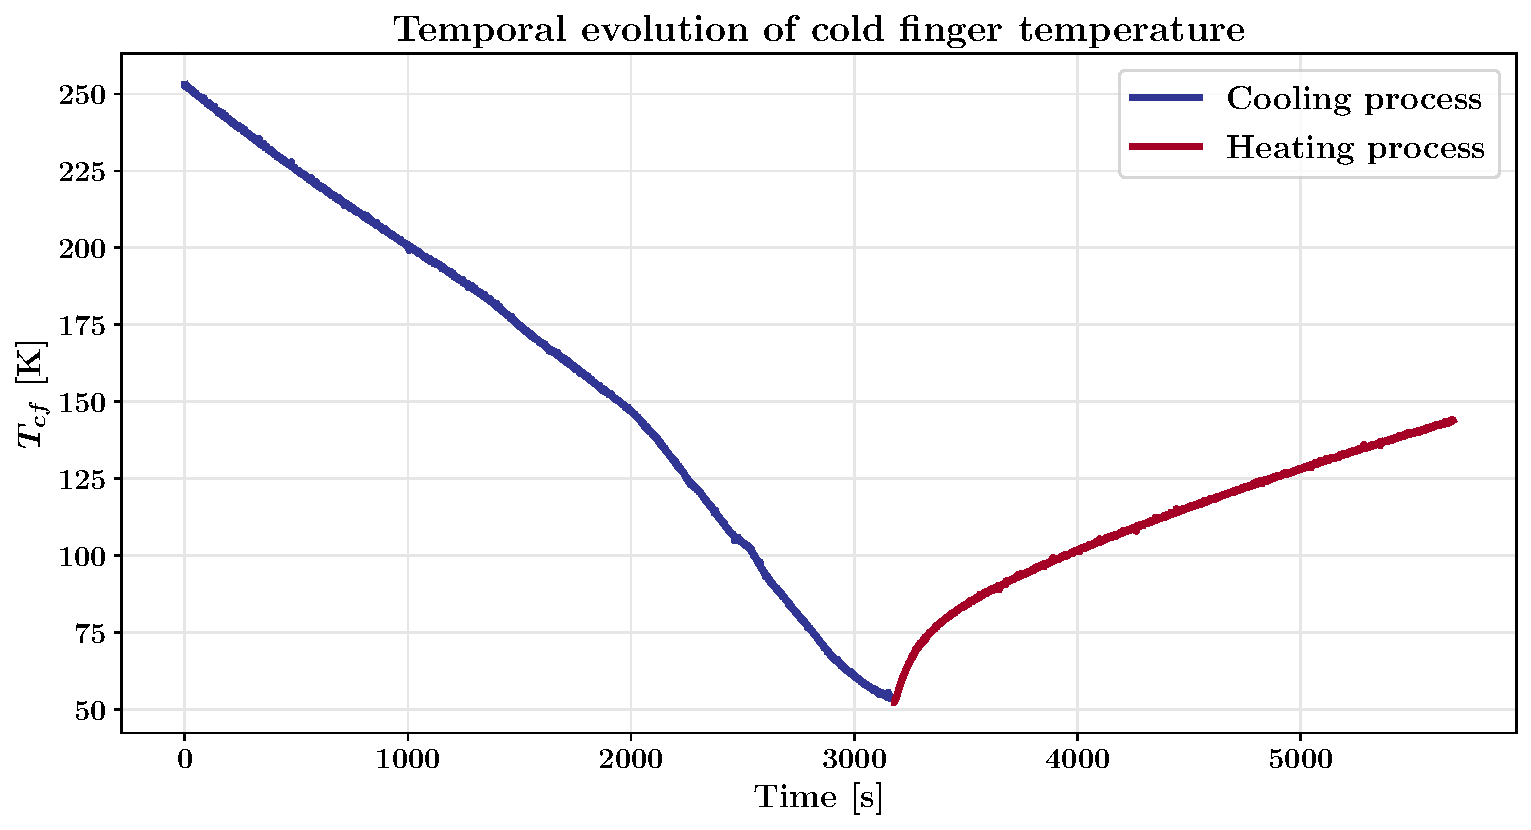
\includegraphics[width=0.85\textwidth]{image/arduino_plots/temporal_evolution_cold_finger.pdf}
    \caption{Temperature of the cold finger $T_{cf}$ as a function of time. The acquisitions starts from the activation of the cryocooler (blue section) and proceeds after its shutdown (red section).}
    \label{fig:cool}
\end{figure}

\subsection{Arduino data}
\label{subsec:arduino_data}

To begin with, the data recorded by the Arduino from the Pt100-cf is studied. As anticipated in SEC. \ref{subsec:arduino_acquisition}, both the Pt100-cf temperature and the output voltage $V_{out}$ are recorded. By matching the timestamps of these two recordings, it is possible to obtain a $V_{out}$ vs $T_{cf}$ plot as shown in FIG. \ref{fig:ardat} for both the cooling and heating processes. 

The AD converter of the Arduino-Uno analog pins reads analog voltages and converts them into digital values; this leads to having a limited resolution of \SI{5}{\milli \volt} in the recorded data. Moreover, the device is set to acquire data at a rate which is much faster than the time required for having significant temperature variations in the system.
For these reasons, this matching procedure might associate more than one value of $V_{out}$ to the same $T_{cf}$. 
This, together with the oscillations in $V_{out}$ leads the data to be quite noisy. To reduce these fluctuations, we associate to each $T_{cf}$ the average value of all the $V_{out}$ recorded at that same temperature. The standard error of the mean is associated to these averaged $V_{out}$.

It can be seen that the range of temperatures investigated during the heating process is smaller than the one for cooling. This is due to the fact that increasing the temperature of the system is very time-consuming as shown in FIG. \ref{fig:cool}. Since measures at higher temperatures are beyond the interest of this study, the acquisition is stopped soon after the observation of the transition back to the normal conductive state.

\begin{figure}[h!]
    \centering
    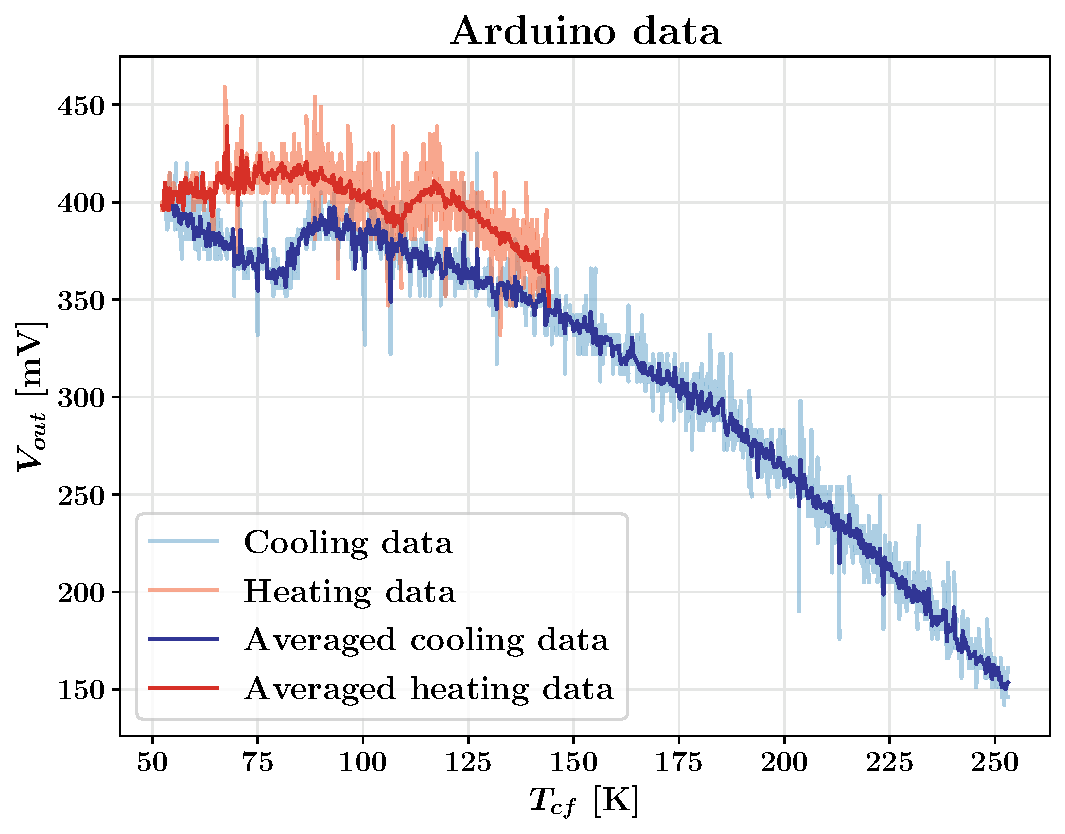
\includegraphics[width=0.7\textwidth]{image/arduino_plots/arduino_data.pdf}
    \caption{Output voltage $V_{out}$ as a function of the temperature of the cold finger $T_{cf}$ in both the cooling and heating processes. The noisy cuves correspond to the raw data from the Arduino whereas the darker, less noisy ones are obtained averaging the $V_{out}$ collected at the same $T_{cf}$.}
    \label{fig:ardat}
\end{figure}


\subsubsection{Comparison with theoretical behaviour}
\label{subsec:comparison_theoretical_behaviour}

One can immediately notice that the data trend in FIG. \ref{fig:ardat} is very different from what is expected from literature. First of all, despite the fact that a net drop in voltage can be distinguished below a certain temperature, this jump is encased in a very strong and distinct background. Because of this, even after the transition to the superconductive state has occurred, the output voltage from the amplifier $V_{out}$ is far from being nil.

This background tension probably originates from the contact potential difference between the different materials composing the circuit: the resistive wires inside the vacuum chamber, the conductive ones in the circuit and the tin solders in the NIM module. At thermal equilibrum in a closed circuit, the sum of these Volta potentials must be zero. As a matter of fact, when testing the response of the amplifier circuit at room temperature (i.e. when the cryocooler was off) this underlying voltage was not detected at all, and the experimental output matched the one expected (see SEC. \ref{subsec:amplifier_circuit}). However, during both the cooling and heating process, the system is not at equilibrium, and the temperature gradients across its components generate this thermoelectric electromotive force due to Seebeck effect \cite{mazzoldi2002fisica}. The main contribution to this voltage arises at the feedthrough of the cryostat where the resistive wires inside are connected to the conductive ones outside at room temperature. For this reason, the entity of this electromotive force is probably further enhanced by the amplifier circuit.

In light of this, the presence of these contact potentials has an effect similar to having in series to the input of the amplifier circuit a voltage generator with temperature-gradient-dependent output, adding an ulterior contribution to $V_{in}$ without affecting $V_{SC}$. However, since the temperature gradient at the feedthrough cannot be eliminated nor controlled, the reproducibility of our measures is negatively influenced. Indeed, the absolute value of $V_{out}$ turns out to be not consistent across different runs, even with same input voltage $V_0$ and at the same absolute temperature $T$ of the sample. Thankfully, this is not a problem since the value of $T_c$ where the voltage drop occurs is not affected for the reasons previously exposed.

Another deviation from the ideal behaviour is in the fact that, as visible in FIG. \ref{fig:ardat}, the temperatures at which the voltage drop occurs is not consistent between the heating and cooling processes. The reason behind this discrepancy is that the Pt100-cf, as already stated in SEC. \ref{sec:experimental_setup}, is coupled to the cold finger. Consequently, it registers a systematically lower temperature with respect to the actual one of the sample. 

Finally, we can observe that, as anticipated in SEC. \ref{sec:introduction} the transition is not perfectly sharp but it is spread over a non negligible range of about $\sim \SI{10}{\kelvin}$.


\subsubsection{Estimate of the critical temperature}
\label{subsubsec:arduino_estimate_critical_temperature}

In spite of the problems exposed in SEC. \ref{subsec:comparison_theoretical_behaviour}, it is still interesting to try and estimate $T_c$ also from this data. The results of this analysis will be useful in SEC. \ref{subsubsec:correction_arduino} where the delay of the sample with respect to the cold finger is quantified by comparison with the Pt100-s data.

To obtain a rough evaluation of the temperature at which the transition is terminated, we interpolate with two lines the data before and after the minimum of the jump in tension, and estimate $T_c$ as the crossing point of these two lines. The parameters of the four lines derived from this fitting procedure are depicted in FIG. \ref{tab:arduino_fit_dat} for both the cooling and heating processes. Moreover, the estimates of the crossings are also reported. The interpolating lines and corresponding residuals are reported in FIG. \ref{fig:ard_Tc}. 
Recalling the averaging process described in SEC. \ref{subsec:arduino_data}, the error associated to the resulting averaged voltages is the standard error of the mean. On the other hand, when only one value of $V_{out}$ was collected for a certain $T_{cf}$ the resolution of the Arduino is taken as maximum error  (\SI{5}{\milli \volt}). 

Furthermore, since the signal-to-noise ratio is a lot worse for the acquistion of $V_{out}$ than it is for $T_{cf}$, in this fit the errors on the abscissae are neglected. 

Moreover, for the computation of the error of the crossings between the interpolating lines, it is essential to consider the covariance terms in the propagation of random errors since the correlation between parameters obtained from the same fit are not negligible.


    \begin{table}[H]
    \sisetup{separate-uncertainty}
    \begin{tabular*}{\linewidth}{@{\extracolsep{\fill}}
    l 
    l 
    S[table-format=3(1)]  %intercept
    S[table-format=1.2(2)] %slope
    S[table-format=1.3]
    l 
    l 
    c 
    c  
    }
        \toprule
    & \textbf{Linear fit} & \textbf{ Intercept [mV] }  & \textbf{ Slope [mV/K] } & $\pmb{r}$ & \textbf{$\pmb{\chi^{(2)}}$/ndf} & \textbf{p-value} & \textbf{$\pmb{T_c}$ [K]} & \textbf{$\pmb{V(T_c)}$ [mV]}\\
        \colrule
    \multirow{2}{*}{{\color{cool}\textbf{Cooling}}} & $\pmb{a_l + b_l \, x }$ &  453\pm3   &   -1.11\pm0.04 & -0.845 & 198.3/61 & $2 \cdot 10^{-16}$ & \multirow{2}{*}{ \tablenum{80\pm1}} & \multirow{2}{*}{ \tablenum{ 363\pm5} } \\
     & $\pmb{a_r + b_r \, x }$ &  99\pm22   &  3.3\pm0.3  & 0.896 & 90.36/17 & $5 \cdot 10^{-12}$\\
         \colrule
    \multirow{2}{*}{{\color{hot}\textbf{Heating}}} & $\pmb{a_l + b_l \, x }$ &  521 \pm 5   &   -1.19 \pm 0.05 & -0.940 & 54.72/57 & 0.561 & \multirow{2}{*}{ \tablenum{ 109 \pm 3}} & \multirow{2}{*}{ \tablenum{ 392\pm8} } \\
     & $\pmb{a_r + b_r \, x }$ &  173\pm10   &  2.01\pm0.09  & 0.915 & 47.81/33& 0.046\\ 
    \botrule
    \end{tabular*}
    \caption{Parameters of the linear fits performed on the Arduino data with Pearson coefficient r, $\chi^{(2)}$/ndf and right-tail p-value. In the last two columns, the coordinates of the crossings are also reported. The subscript $l$ refers to the data from the left fits and $r$ to the right ones.}
    \label{tab:arduino_fit_dat}
    \end{table}

As regards the heating data, the values of $\chi^{(2)}$/ndf, are quite close to the expected value of 1. On the other hand, the ones for the cooling fits are much higher than expected. This also translates into very low values of p-value (i.e. the integral at the right of the experimental value of $\chi^{(2)}$ of the theoretical distribution at the correspondent number of degrees of freedom ndf). This is due to an underestimation of the errors associated to the cooling data. Indeed, the standard error of the mean which was associated to these averaged $V_{out}$ is a reasonable estimation of the error for the heating dataset since it is very noisy and thus that average is performed over a greater set of values. On the other hand, since the dataset collected in the cooling process is cleaner, the error of the mean fails to capture the full variability due to the noise. 

These arguments are supported by the residuals shown in FIG. \ref{fig:ard_Tc}. It can be seen that for all four fits, the residuals are randomly dispersed around the zero value, suggesting the absence of systematic errors and justifying the assumption of linearity. However, the compatibility of these residuals with zero is not always optimal, especially with the cooling data for the reasons previously explained.

The presence of a distinct linear correlation in the data is also supported by the values of the Pearson coefficients $r$ which are good (but not excellent especially in the left line for the cooling data). 

Another fact worth mentioning is the entity of the relative error on the intercepts, which is quite considerable especially for the right fits. This is due to the fact that the interpolation of the right portion are performed over a very reduced dataset and quite far from the origin.

Lastly, by looking at the estimates of $T_{c}$ obtained from this method, there is a clear difference of almost $\SI{30}{\kelvin}$ between the heating and cooling results. This was already noticed in SEC. \ref{subsec:comparison_theoretical_behaviour} and prevents from obtaining a final unique and reliable estimate of the critical temperature of the sample.

\clearpage

\begin{figure}[H]
\begin{minipage}[c]{0.49\linewidth}
\subfloat[][$T_c$ from cooling process]{ 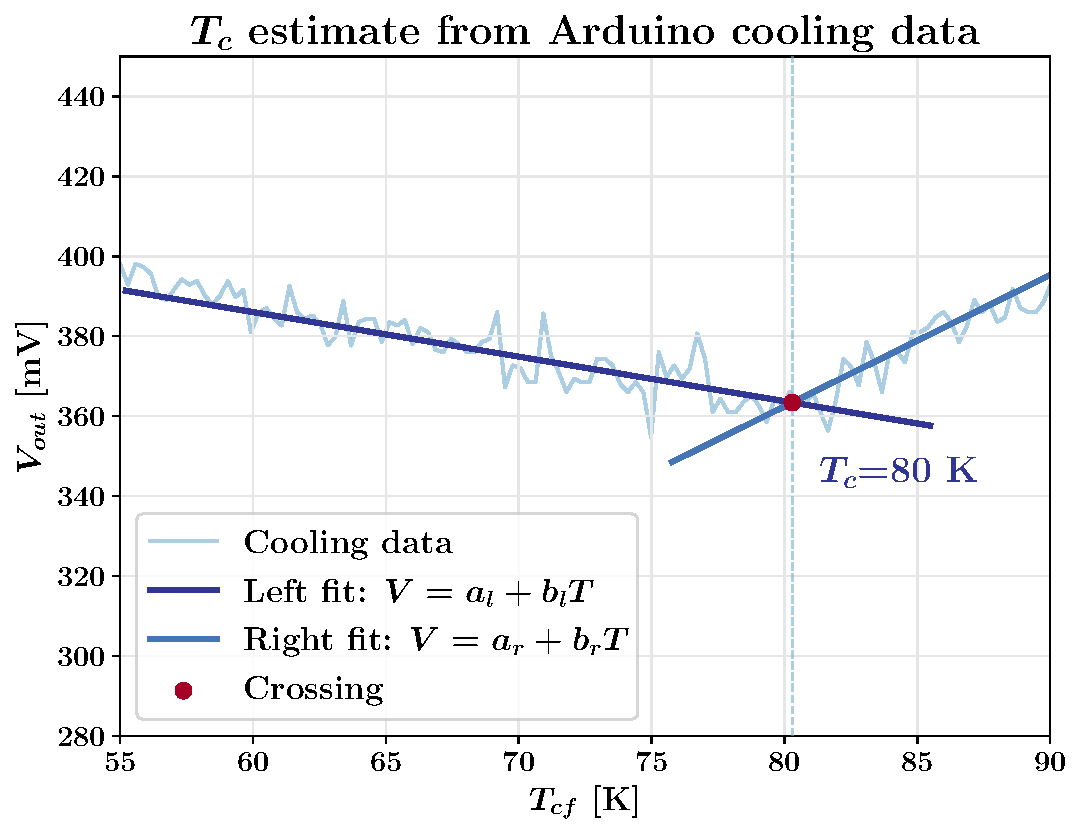
\includegraphics[width=\textwidth]{image/arduino_plots/ard_est_co.pdf} \label{fig:ard_Tc(a)} }
\end{minipage}
\begin{minipage}[]{0.49\linewidth}
\centering
\subfloat[][$T_c$ from heating process]{    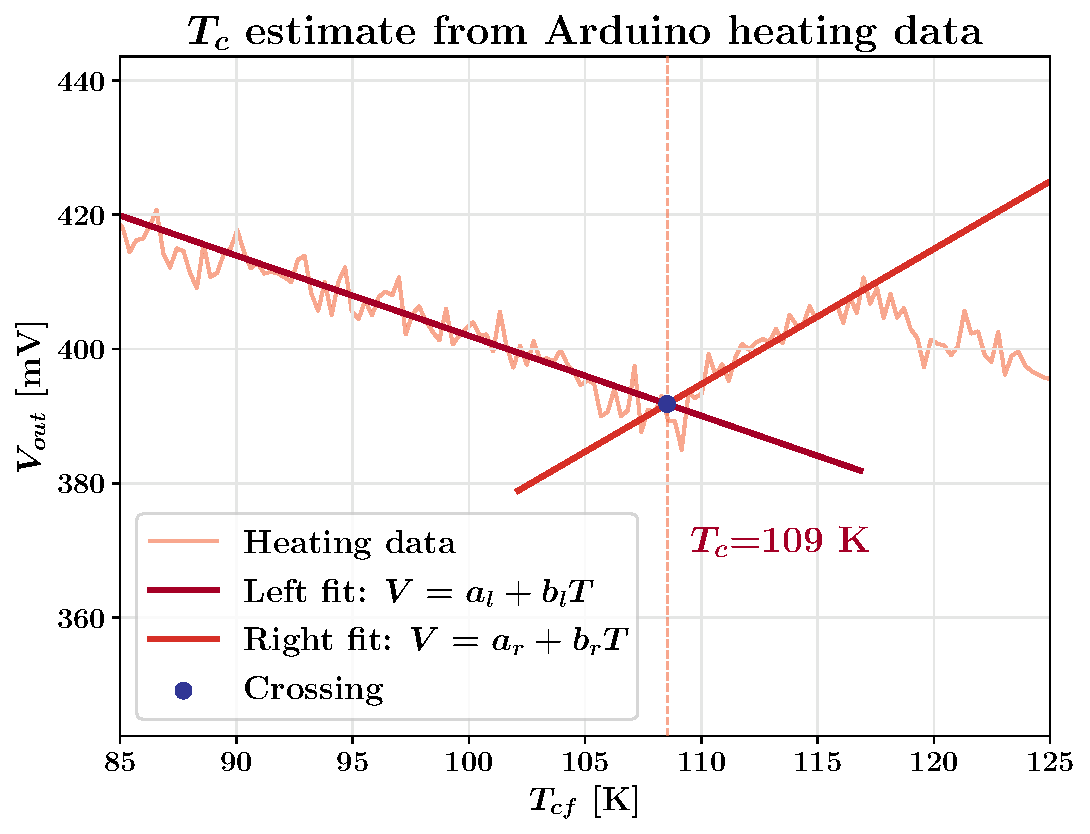
\includegraphics[width=\textwidth]{image/arduino_plots/ard_est_he.pdf}  \label{fig:ard_Tc(b)} }
\end{minipage} \\
\vfill
\begin{minipage}[c]{0.49\linewidth}
\subfloat[][Residuals of left line for cooling]{ 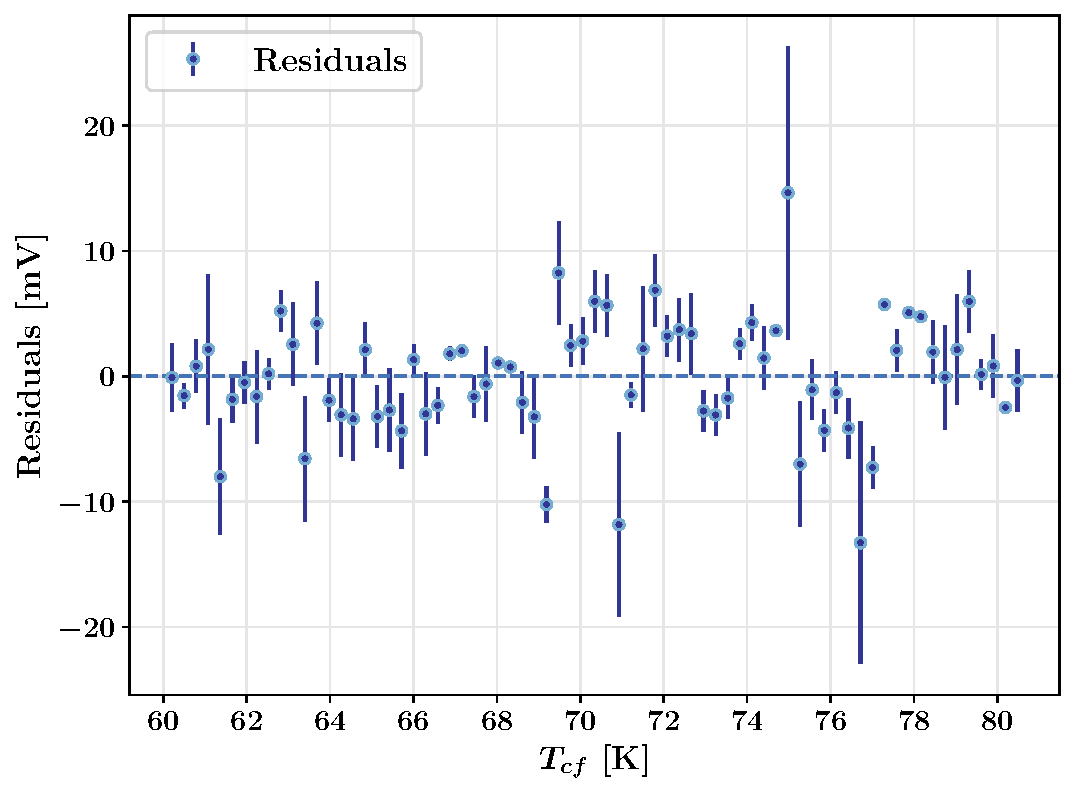
\includegraphics[width=\textwidth]{image/arduino_plots/ard_res_left_co.pdf} \label{fig:ard_Tc(c)} }
\end{minipage}
\begin{minipage}[]{0.49\linewidth}
\centering
\subfloat[][Residuals of left line for heating]{    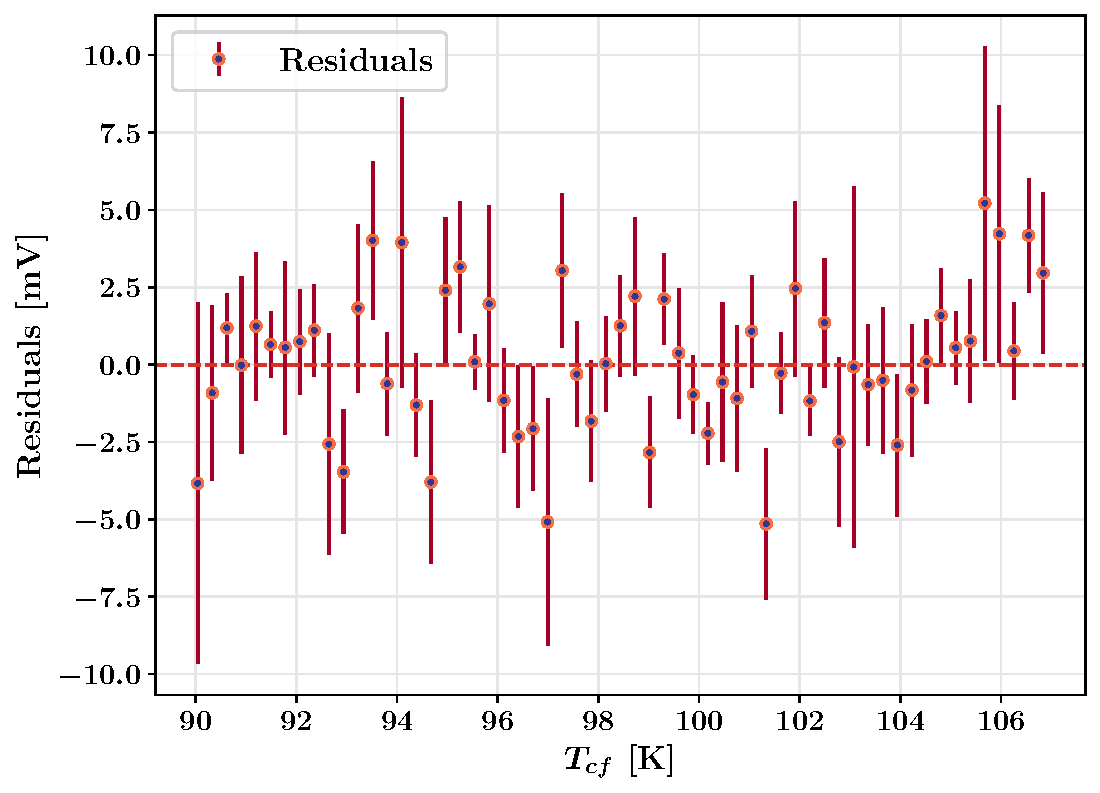
\includegraphics[width=\textwidth]{image/arduino_plots/ard_res_left_he.pdf}  \label{fig:ard_Tc(d)} }
\end{minipage} \\
\vfill
\begin{minipage}[c]{0.49\linewidth}
\subfloat[][Residuals of right line for cooling]{ 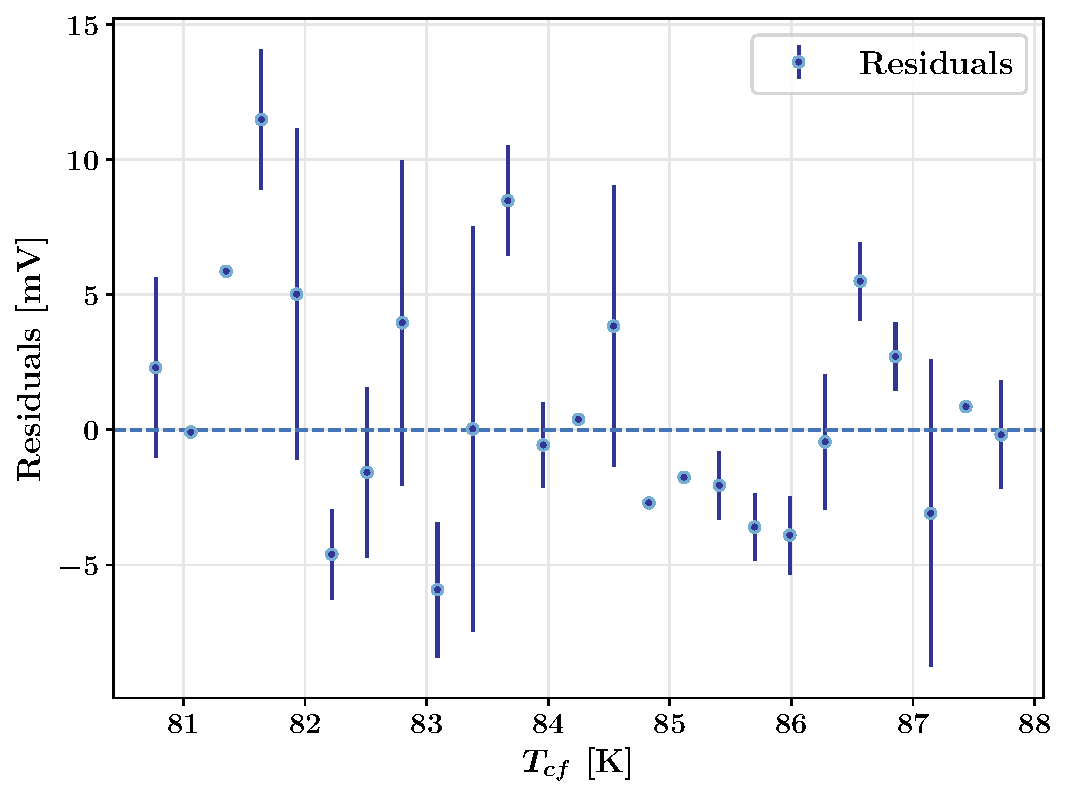
\includegraphics[width=\textwidth]{image/arduino_plots/ard_res_right_co.pdf} \label{fig:ard_Tc(e)} }
\end{minipage}
\begin{minipage}[]{0.49\linewidth}
\centering
\subfloat[][Residuals of right line for heating]{    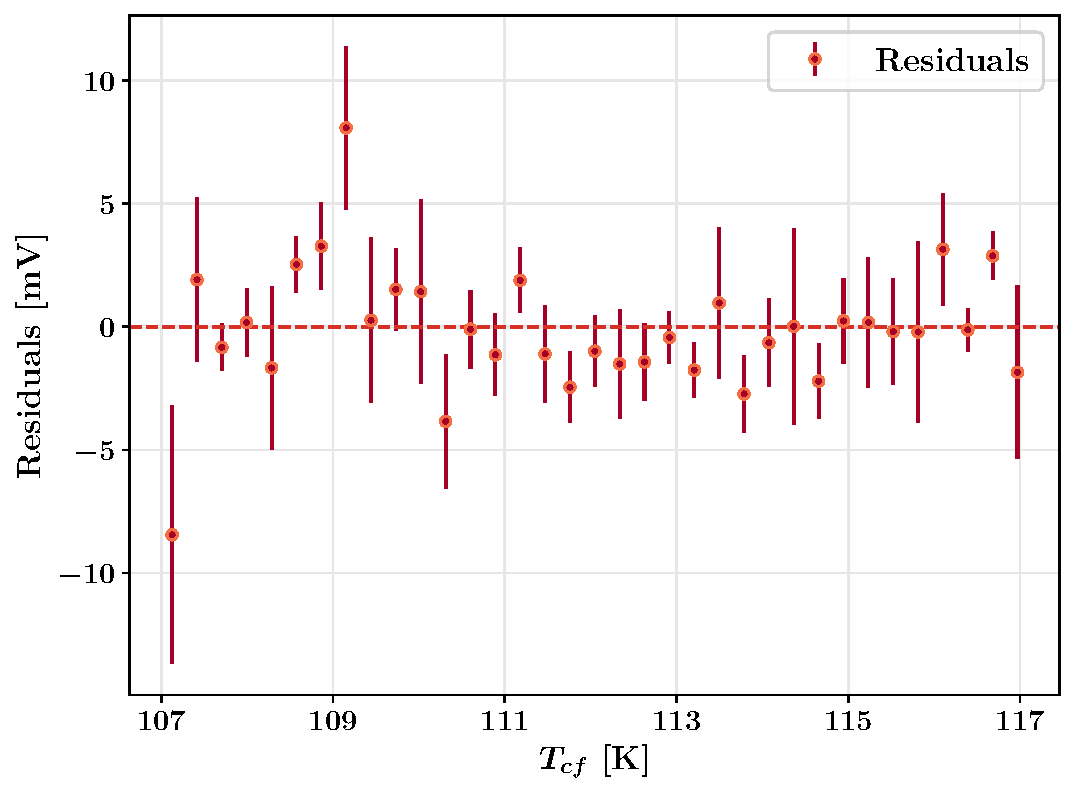
\includegraphics[width=\textwidth]{image/arduino_plots/ard_res_right_he.pdf}  \label{fig:ard_Tc(f)} }
\end{minipage}
\caption{\label{fig:ard_Tc} Estimate of the critical temperature $T_c$ from the data of Pt100-cf connected to the Arduino in both the cooling \ref{fig:ard_Tc(a)} and heating \ref{fig:ard_Tc(b)} processes. Graphs \ref{fig:ard_Tc(c)} and \ref{fig:ard_Tc(e)} show the residuals of two lines used to interpolate the left and right side respectively of the minimum in the cooling data. Graphs \ref{fig:ard_Tc(d)} and \ref{fig:ard_Tc(f)} are the same but for the heating data.}
\end{figure}


\subsection{Manual drift data}
\label{subsec:manual_drift_data}

A more reliable estimate of $T_c$ can be found using the temperature bridge described in SEC. \ref{subsec:thermometer_bridge}, as the Pt100-s is closer to the sample with respect to the Pt100-cf. 


\subsubsection{Uncertainties associated to ($R_T$,$V_{\text{out}}$)}

As already mentioned in \ref{subsec:manual_drift_acquisition}, the thermal bridge gives only an indirect access to the resistance of the platinum thermometer through the helipot one $R_v$ set to satisfy the balance condition. The value of $R_v$ can be converted into $R_T$ by using EQ. \eqref{eq:Rt}. According to it, the error in the determination of $R_T$ depends on the errors on $R_1$, $R_2$ and on the uncertainty in the balancing of the bridge $\sigma_{R_v}$.  

Given the number of divisions per turn of the helipot, we assume to be able to distinguish $\sim$ \SI{0.2}{\ohm} in the measurement of $R_v$ with uniform distribution in this interval. Moreover, the gain of the lock-in amplifier is set to a value high enough that by turning the helipot by a single division (\SI{0.2}{\ohm}) the bridge's balance is broken, but low enough that balancing the bridge is still possible. Thus, we are exploiting the full sensitivity offered by the system and can assume $\sigma_{R_v}= 0.2/\sqrt{12} \, \si{\ohm}$. Then, by propagation of errors, we compute the error $\sigma_{R_T}$ of each $R_T$.

Moreover, the error associated to the voltage measurement is given by the multimeter specification at the full-scale of \SI{600}{\mV}. 


\subsubsection{Pt100 conversion curve}
\label{sec:Pt100_conversion_curve}

To convert $R_T$ into a temperature measure, one can make use of the calibration table of the platinum thermometer.

Since the Pt100 temperature and its resistance are with good approximation linearly proportional to each other (as seen in SEC. \ref{subsec:thermometer_bridge}), we perform a linear fit  of the tabulated data in the range of interest of $[70,160]\,\si{\kelvin}$ to find a conversion formula. 

The calibration data and its interpolating curve are shown in FIG. \ref{gra:Pt100cal}, together with the residuals. One can notice that the trend is highly non-linear for low resistances. These correspond to temperatures which are outside our range of interest and are thus rejected in the fit procedure.  

The fit of calibration data is performed considering errors on both the $x$ and $y$ coordinates. The calibration datasheet only provides the ratio between the maximum uncertainties $\frac{\Delta R}{\Delta T \cdot 100}$. Thus, one can derive the error on the temperature from the one on the resistance. 

Since the relative error of the $R_T$ measured was found to be approximately the same for all $R_T$, at about $0.7\%$, $\sigma_R$ was calculated taking this value as relative error also for the $R$ on the datasheet. Finally, $\sigma_T$ is derived from the corresponding $\sigma_R$. With this estimate, the relative errors on the $T$ also turn out to be approximately constant at about $0.4 \%$.

\begin{table}[H]
    \centering
    \sisetup{separate-uncertainty}
    \begin{tabular*}{0.8\linewidth}{@{\extracolsep{\fill}}
    l 
    S[table-format=2.1(1)]  %intercept
    S[table-format=1.3(3)] %slope
    l%S[table-format=1.5]
    l 
    l 
    }
        \toprule
     \textbf{Linear fit} & \textbf{Intercept [K]}  & \textbf{Slope [K/$\pmb{\Omega}$]} & $\pmb{r}$ & \textbf{$\pmb{\chi^{(2)}}$/ndf} & \textbf{p-value} \\
        \colrule
     $\pmb{a + b \, x }$ &  33.6\pm0.1   &   2.323\pm0.005 & 0.99998 & 8.003/357 &  1 \\
    \botrule
    \end{tabular*}
    \caption{Parameters of the linear fit of the Pt100 conversion data with Pearson coefficient r, $\chi^{(2)}$/ndf and p-value.}
    \label{tab:Pt100cal_fit_dat}
\end{table}

The Pearson coefficient highlights the very high level of linear correlation of the data. However, by looking at the residuals, it can be seen that they are not randomly scattered around zero but they show a parabolic trend for the higher values of R. This is due to the fact that the linear dependence expressed in EQ. (\ref{eq:ResTPt100}) is an approximation. In particular the value of $\alpha$ might not be exactly constant with the temperature. Nonetheless, in the range of temperatures considered for the experiment, the theoretical model can be assumed with overall good approximation.

The $\chi^{(2)}$ is very small compared to the number of degrees of freedom. Consequently, the p-value turns out to be basically equal to the full integral of the distribution curve. This highlights a big overestimation of the errors. This is especially true for the data at lower values of $R$, where the theoretical linear behaviour is followed quite accurately. Since most of the interpolated data falls in this region, they strongly affect the estimate of $\chi^{(2)}$. However, by looking at the residuals, we can see that in order for the data with $R>\SI{40}{\ohm}$ to be compatible with the line, the error associated is reasonable.

\begin{figure}[H]
\begin{minipage}[c]{0.49\linewidth}
\subfloat[][Pt100 conversion fit]{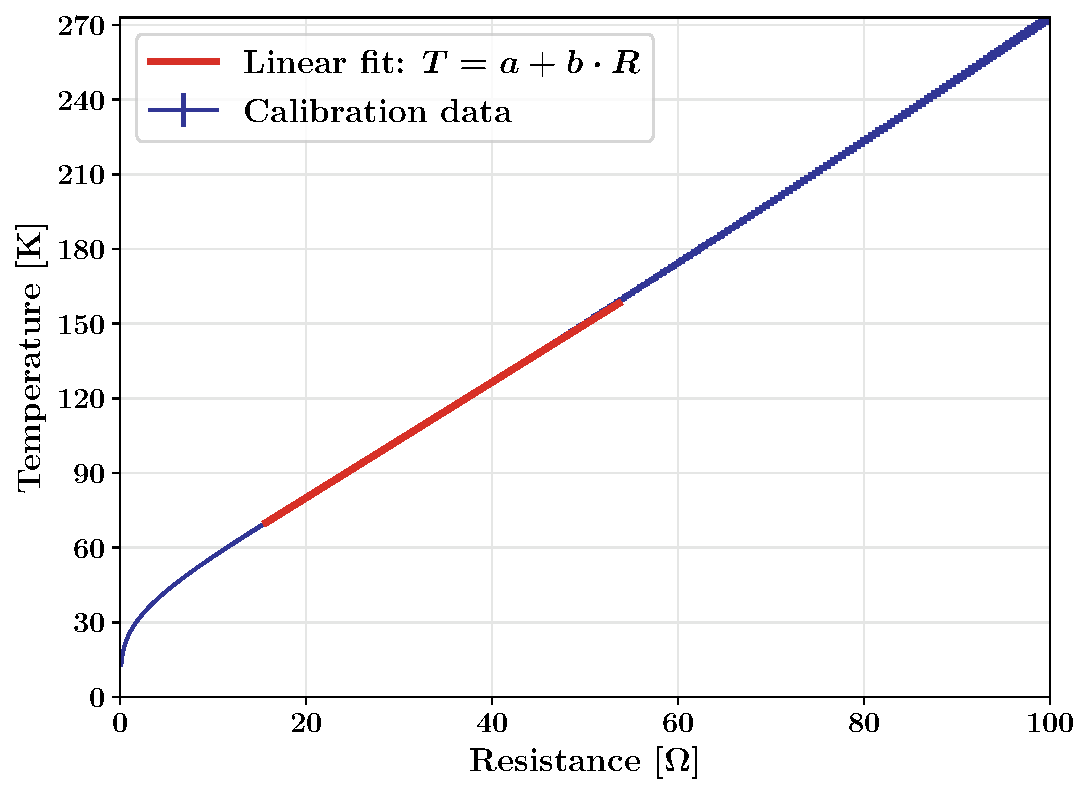
\includegraphics[width=\textwidth]{image/drift_plots/Pt100_conversion.pdf} \label{gra:Pt100cal_fit} }
\end{minipage}
\begin{minipage}[]{0.49\linewidth}
\centering
\subfloat[][Residuals of fit]{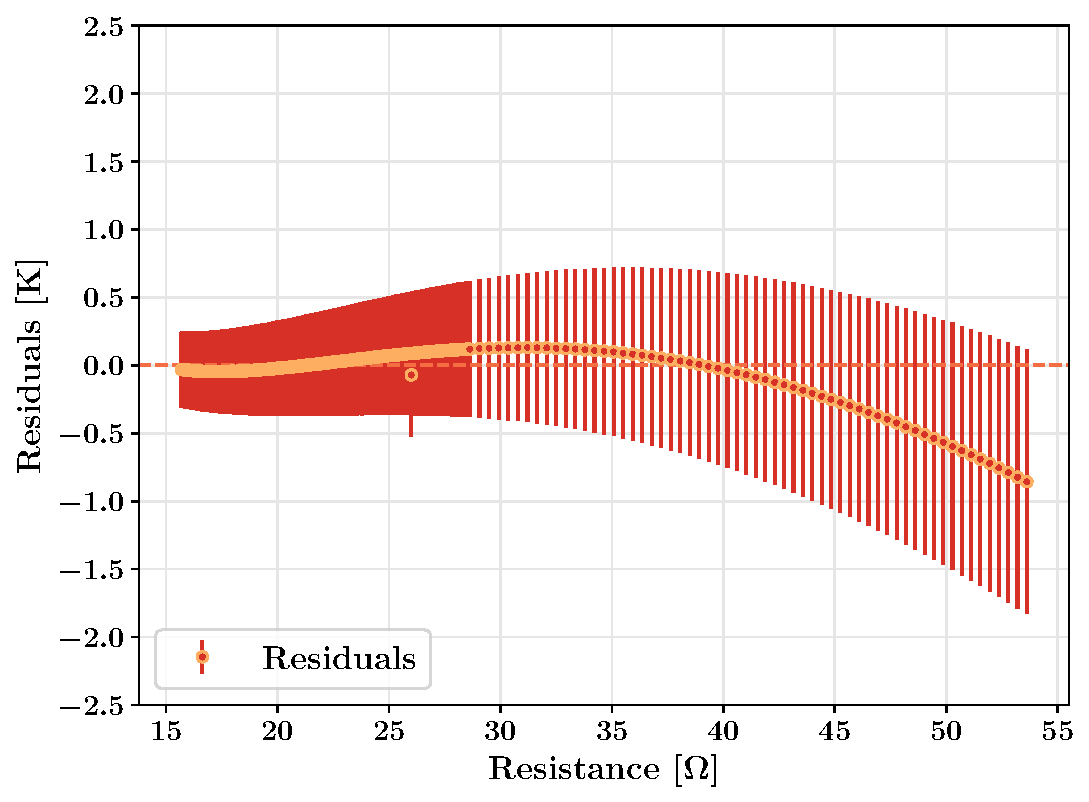
\includegraphics[width=\textwidth]{image/drift_plots/Pt100_res.pdf}  \label{gra:Pt100cal_res} }
\end{minipage}
\caption{\label{gra:Pt100cal} In \ref{gra:Pt100cal_fit} the Pt100-s calibration data and interpolating line for conversion in temperature are illustrated, while \ref{gra:Pt100cal_res} shows the corresponding residuals. }
\end{figure}


\subsubsection{Analysis of drift measurements}
\label{subsubsec:drift_measurement}

In FIG. \ref{fig:mandat} the data recorded using the three-wire bridge described in SEC. \ref{subsec:thermometer_bridge} is shown. The errors on $T_s$ are calculated by error propagation from the Pt100-s  calibration line in SEC. \ref{sec:Pt100_conversion_curve}. 

\begin{figure}[H]
    \centering
   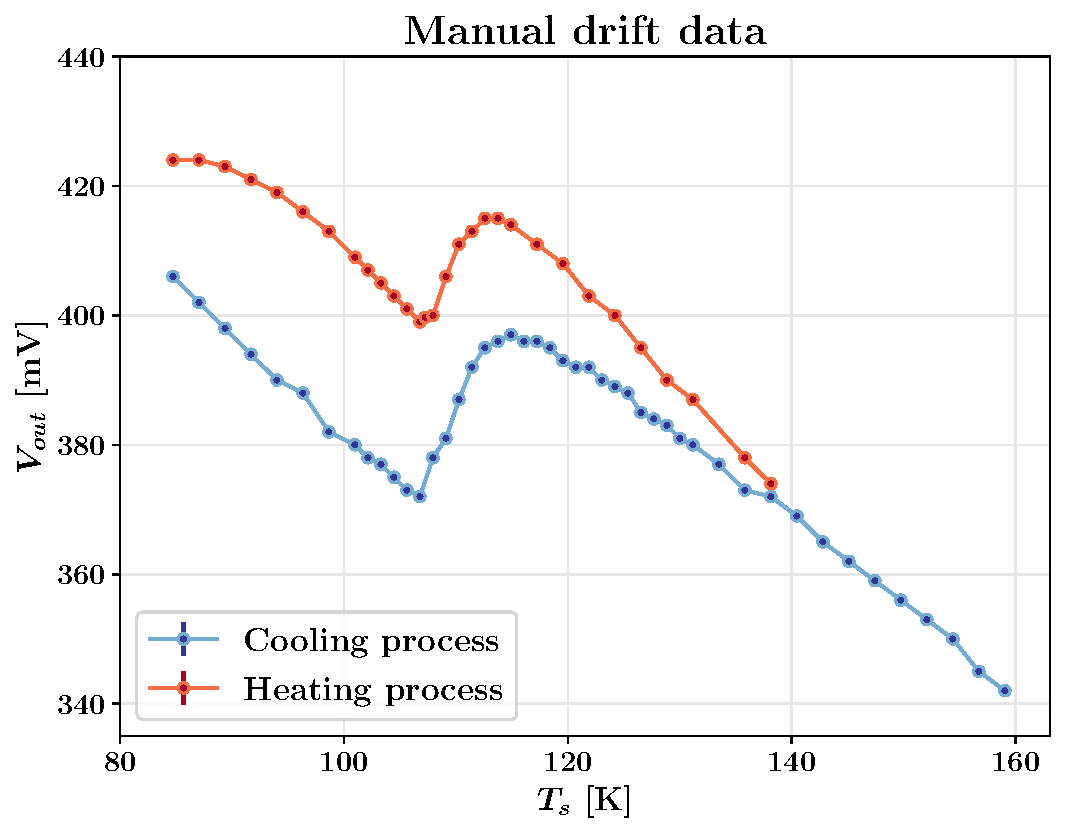
\includegraphics[width=0.7\textwidth]{image/drift_plots/drift_data.pdf}
    \caption{Output tension from the amplifier connected to the sample as a function of $T_s$, temperature of the Pt100-s, in both the cooling and heating processes.}
    \label{fig:mandat}
\end{figure}

\pagebreak

One can immediately notice the absence of the hysteresis between cooling and heating that was observed in the Arduino data. This proves that the coupling of Pt100-s with the sample is good and that the power dissipated on the sample itself is indeed negligible, as anticipated in SEC. \ref{subsec:amplifier_circuit}. 
 
However, the background voltage is still present. Since the data is less noisy than the one collected using the Arduino, we can try to remove this background $V_{off}$ and isolate the actual amplified tension across the sample $\Delta V_{out} = V_{out} - V_{off}$. 
To accomplish the removal of this thermoelectric electromotive force, we interpolate the left side of the step (where $\Delta V_{out}$ should be zero) with a line $a_b + b_b x$ that is then subtracted from the rest of the data. However, the background does not display a univocal trend given its strong dependence on the temperature gradients. For this reason, we must restrict the range of interpolation to the region in close proximity to the transition. This will lead to quite big errors especially in the intercept. 

Once that $\Delta V_{out}$ is isolated, it can also be converted into a resistance, using the constant current approximation EQ. \eqref{eq:I_const} and dividing by the amplifier gain $G$ as in EQ. \eqref{eq:R_SC_estimate}. The errors are obtained by propagation of errors due to both the subtraction of the line interpolating the background and to EQ. (\ref{eq:R_SC_estimate}).

After this, the trend of the data resembles more closely the one theoretically predicted aside from some non-physical results like negative resistances in the leftmost portion of the curve and decrease of resistivity in the normal conductive region. These are due to the random behaviour of the underlying electromotive force and the fact that only the left portion in close proximity to the transition was considered for the background interpolation. This is especially visible in the heating data where the linear approximation of the background was not as good as in the cooling. For these reasons, as before, we estimate $T_c$ as the temperature at which the transition is completed and the sample fully behaves as a superconductor.  
Thus, we also interpolate the transition region with a line $a_t + b_t x$ and then find $T_c$ as its crossing with the background level $y=0$.

The results of this analysis can be observed in the graphs in FIG. \ref{fig:drift_co} and \ref{fig:drift_he}.
The residuals for $a_b + b_b x$ are in FIG. \ref{fig:drift_co_res_bg}, \ref{fig:drift_he_res_bg}, while those for $a_t + b_t x$ are in FIG. \ref{fig:drift_co_res}, \ref{fig:drift_he_res}. 
In TAB. \ref{tab:drift_fit_dat} we list the parameters of these fits. The crossing $T_c$ with $y=0$ is also reported in the same table.

 \begin{table}[H]
    \sisetup{separate-uncertainty}
    \begin{tabular*}{\linewidth}{@{\extracolsep{\fill}}
    l 
    l 
    S[table-format=3(1)]  %intercept
    c@{\hskip 0.3in}
    S[table-format=1.2(2)] %slope
    c@{\hskip 0.3in} %S[table-format=1.3]
    c
    l 
    l 
    c%S[table-format=1.3] 
    }
        \toprule
    & \textbf{Linear fit} & \textbf{Intercept}  & & \textbf{Slope} & & $\pmb{r}$ & \textbf{$\pmb{\chi^{(2)}}$/ndf} & \textbf{p-value} & \textbf{$\pmb{T_c}$ [K]}\\
        \colrule
    \multirow{2}{*}{{\color{cool}\textbf{Cooling}}} & $\pmb{a_b + b_b \, x }$ &  536\pm2 & [mV] & -1.55\pm0.02 & [mV/K] & -0.998 & 30.05/11 & 0.002 & $-$ \\
     & $\pmb{a_t + b_t \, x }$ & -181\pm17 & [m$\Omega$] & 1.7\pm0.2 & [m$\Omega$/K]  & 0.993 & 1.62/5 & 0.899 & \tablenum{106.4\pm 0.4} \\
         \colrule
    \multirow{2}{*}{{\color{hot}\textbf{Heating}}} & $\pmb{a_b + b_b \, x }$ &  576\pm5 & [mV] & -1.65\pm0.05 & [mV/K] & -0.9990 & 1.97/6 & 0.922 & $-$ \\
     & $\pmb{a_t + b_t \, x }$ & -168\pm32 & [m$\Omega$] & 1.6\pm0.3 & [m$\Omega$/K]  & 0.991 & 0.550/4 & 0.968 & \tablenum{107.0 \pm 0.6} \\ 
    \botrule
    \end{tabular*}
    \caption{Parameters of the linear fits performed on the background of the manual drift data ($a_b+b_b x$) and on the region of transition ($a_t+b_t x$) for the cooling and heating processes. The Pearson coefficient $r$, $\chi^{(2)}$/ndf and right-tail p-value are also listed. In the last column, the x-coordinate of the crossings with the background level $y=0$.}
    \label{tab:drift_fit_dat}
    \end{table}


As regards $a_b + b_b x$, the values of $\chi^{(2)}$/ndf are not too far from the optimal value of 1 but they still highlight a slight underestimation of the error for the cooling data and an overestimation for heating. This can be noticed also by looking at the residuals (FIG. \ref{fig:drift_co_res_bg}, \ref{fig:drift_he_res_bg}). The latter also show that assuming a linear behaviour for the underlying electromotive force is quite rough since their placement around zero is not completely randomic. Nonetheless, it is quite difficult to establish a priori a model for this tension. Moreover, increasing the complexity of the fit function, would lead to data overfitting. In light of this, we choose to limit ourselves to a linear model for the sake of simplicity. 

Concerning $a_t + b_t x$, the values of $\chi^{(2)}$/ndf are bit small due to overestimation of the errors caused by the big relative error on the parameters of the background fit. This is supported by the fact that the smallest $\chi^{(2)}$/ndf is the one for the heating data, where less points are considered causing a bigger uncertainty. Moreover, the residuals (FIG. \ref{fig:drift_co_res} and \ref{fig:drift_he_res}) are in both cases randomly dispersed around zero and compatible with it, justifying the linear model.

The Pearson coefficients $r$ highlight in all cases a good level of linear correlation in the data.

Regarding the estimates of $T_c$ obtained from this method we can see that the hysteresis is indeed not observable, as the two values are compatible within their experimental error with compatibility $\lambda = 0.83$. Given their compatibility, one can take as final estimate of the critical temperature the weighted average of the two $T_c$ from heating and cooling:
\begin{equation*}
    T_c^{drift} = (106.8 \pm 0.2) \, \si{\kelvin}
\end{equation*}

It is also worth noticing is that, as it can be seen from FIG. \ref{fig:drift_co} and \ref{fig:drift_he}, the order of magnitude of $R_{SC}$ before the superconductor transition is $R_{SC} \approx 0.01 \si{\ohm}$ as anticipated in SEC. \ref{subsec:amplifier_circuit}.


\begin{figure}[h!]
\begin{minipage}[c]{0.49\linewidth}
\subfloat[][Cooling data with subtracted background]{  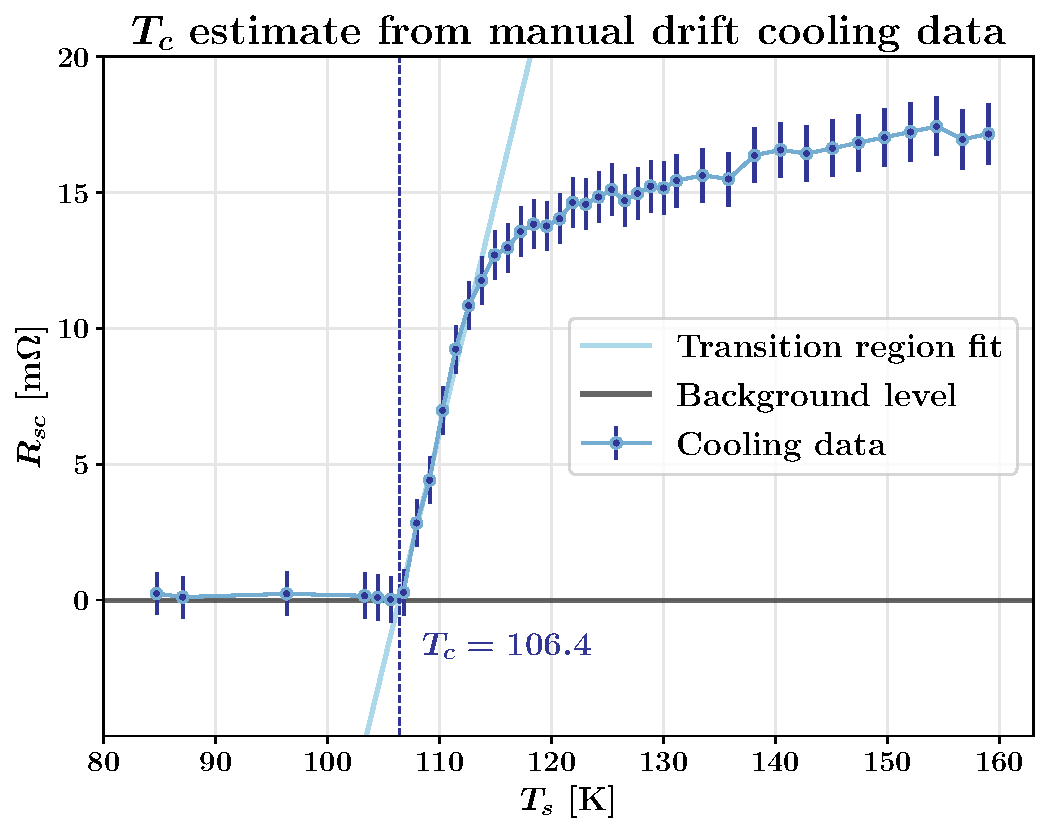
\includegraphics[width=\textwidth]{image/drift_plots/drift_tc_co.pdf} \label{fig:drift_co} }
\end{minipage}
\hfill
\begin{minipage}[]{0.49\linewidth}
\centering
\subfloat[][Heating data with subtracted background]{    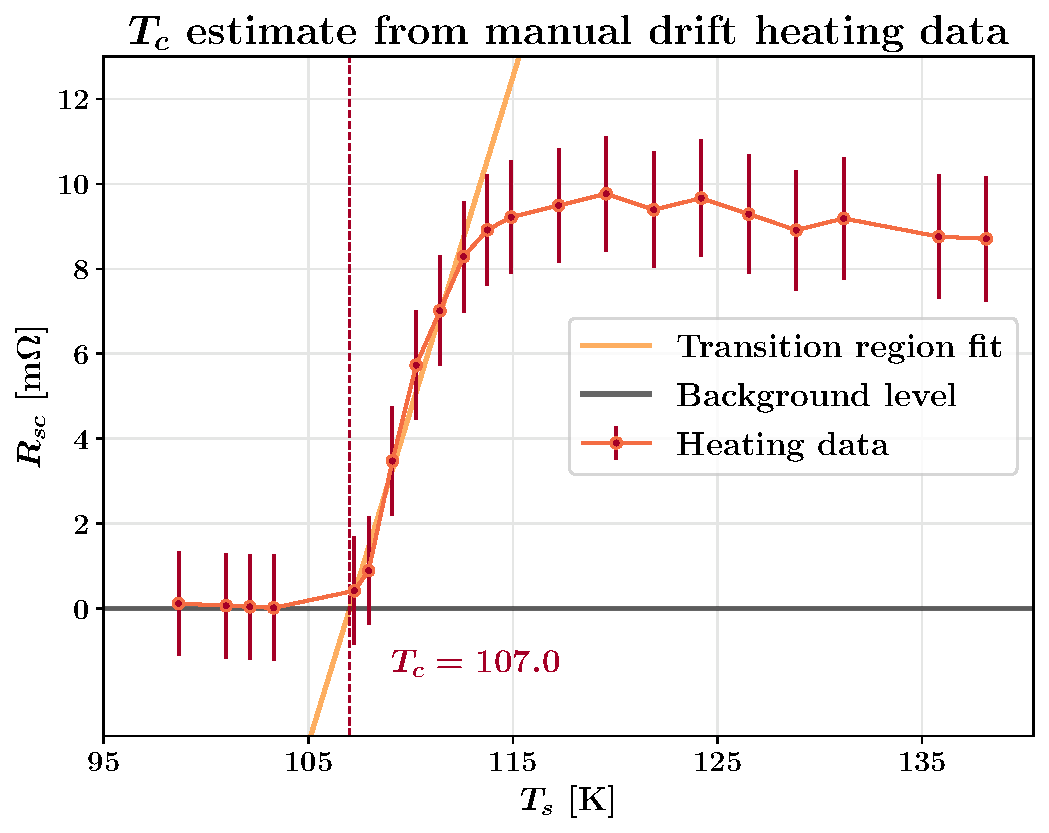
\includegraphics[width=\textwidth]{image/drift_plots/drift_tc_he.pdf}  \label{fig:drift_he} }
\end{minipage}
\begin{minipage}[c]{0.49\linewidth}
\subfloat[][Residuals of linear fit of the background for cooling data]{  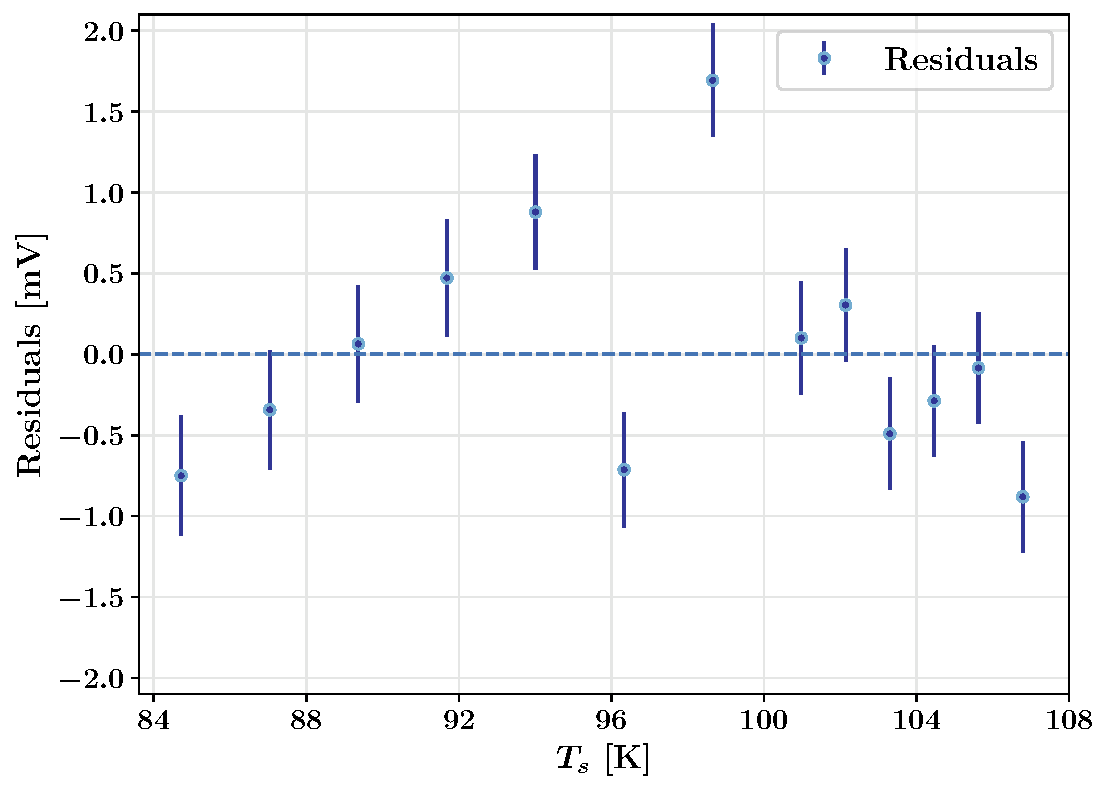
\includegraphics[width=\textwidth]{image/drift_plots/drift_background_res_co.pdf} \label{fig:drift_co_res_bg} }
\end{minipage}
\hfill
\begin{minipage}[]{0.49\linewidth}
\centering
\subfloat[][Residuals of linear fit of background for heating data]{    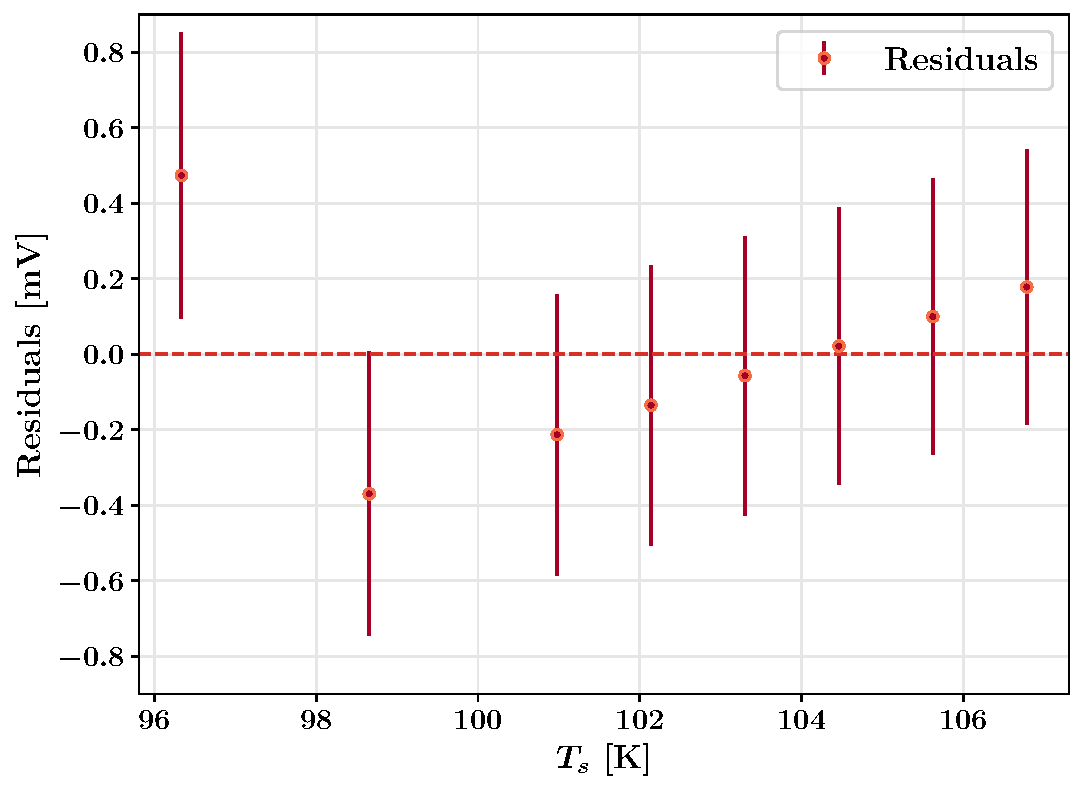
\includegraphics[width=\textwidth]{image/drift_plots/drift_background_res_he.pdf}  \label{fig:drift_he_res_bg} }
\end{minipage}
\begin{minipage}[c]{0.49\linewidth}
\subfloat[][Residuals of linear fit in the transition region for cooling data]{  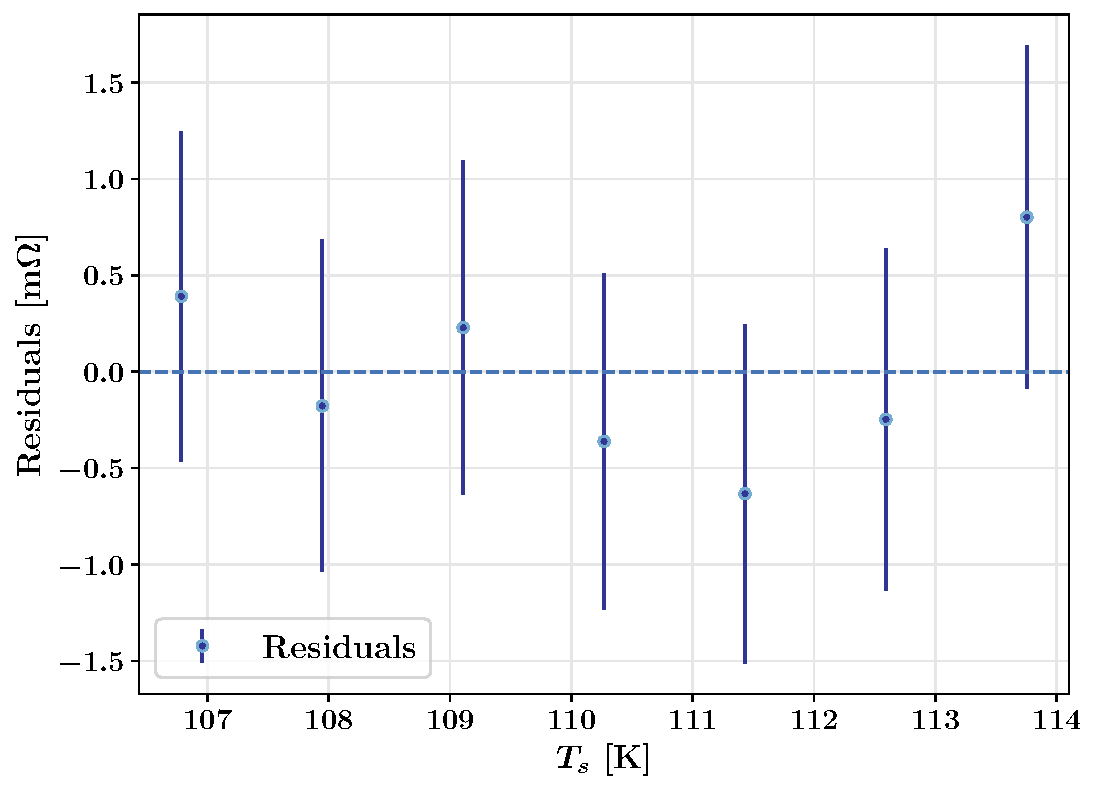
\includegraphics[width=\textwidth]{image/drift_plots/drift_tc_res_co.pdf} \label{fig:drift_co_res} }
\end{minipage}
\hfill
\begin{minipage}[]{0.49\linewidth}
\centering
\subfloat[][Residuals of linear fit in the transition region for heating data]{    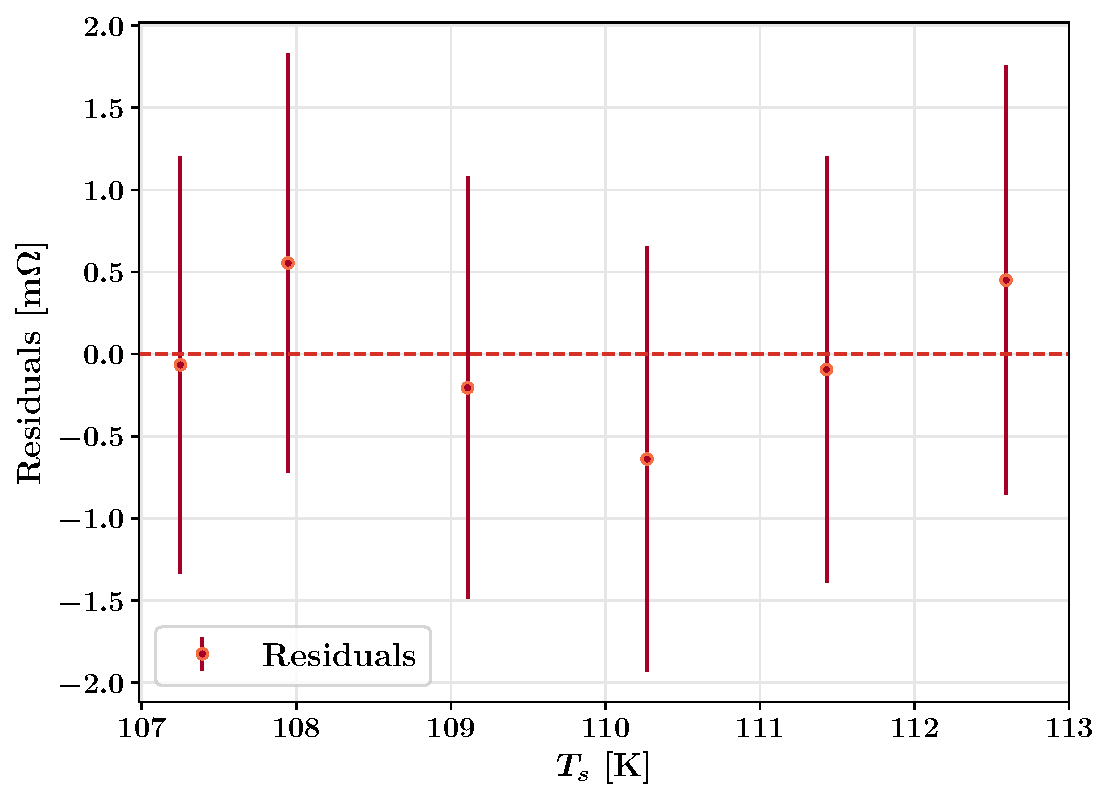
\includegraphics[width=\textwidth]{image/drift_plots/drift_tc_res_he.pdf}  \label{fig:drift_he_res} }
\end{minipage}
\caption{\label{fig:manual_drift} Estimate of the critical temperature $T_c$ from the Pt100-s data subtracting the background voltage interpolated with a linear fit. FIG. \ref{fig:drift_co} and \ref{fig:drift_he} show the resistance of the sample as a function of its temperature in both the cooling and heating processes. FIG. \ref{fig:drift_co_res}, \ref{fig:drift_he_res}, \ref{fig:drift_co_res_bg}, \ref{fig:drift_he_res_bg} are the residuals of the four fits.}
\end{figure}

\clearpage

\subsubsection{Correction of Pt100-cf delay}
\label{subsubsec:correction_arduino}

In light of these results, one can try to correct the systematic error of the Arduino measures due to the bad thermal coupling of Pt100-cf with respect to the sample. In order to do this, we can consider temperature recordings acquired in parallel with both Pt100-cf and Pt100-s and map the temperatures $T_{cf}$ into the correspondent $T_s$ measured at the same instant. 

The result of this mapping is shown in FIG. \ref{fig:Tcf_vs_Ts}. In the range of temperatures of interest, for both the cooling and heating data, the relationship between the two $T$ can be interpolated with good approximation with a line. This procedure is carried out neglecting the errors on $T_{cf}$ and considering only those on $T_{s}$. In FIG. \ref{fig:res_cool_delay} and \ref{fig:res_hot_delay} are depicted the residuals of the two lines. In TAB. \ref{tab:arduino_correction} are the fit parameters.

\begin{figure}[h!]
\begin{minipage}[c]{0.7\linewidth}
\subfloat[$T_{cf}$ vs $T_s$]{ 
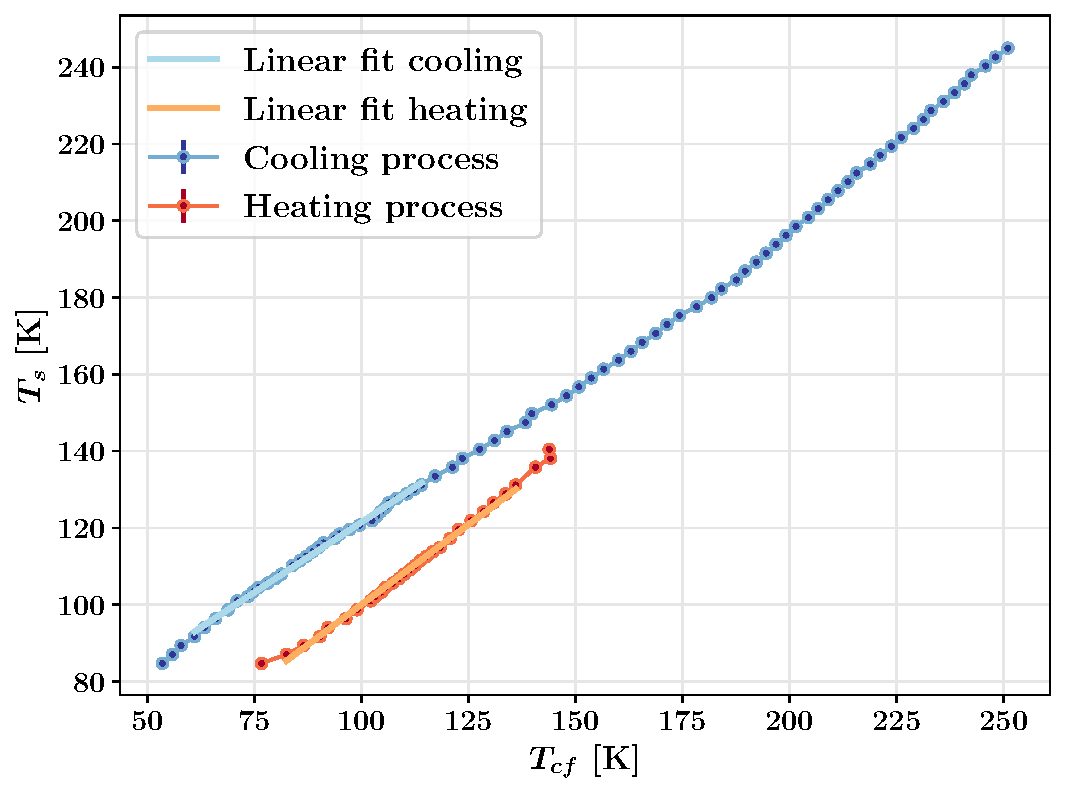
\includegraphics[width=\textwidth]{image/relation_plots/relation_t.pdf} \label{fig:Tcf_vs_Ts} } 
\end{minipage} \\
\vspace{0.5cm}
\begin{minipage}[c]{0.49\linewidth}
\subfloat[Residuals of cooling interpolation]{  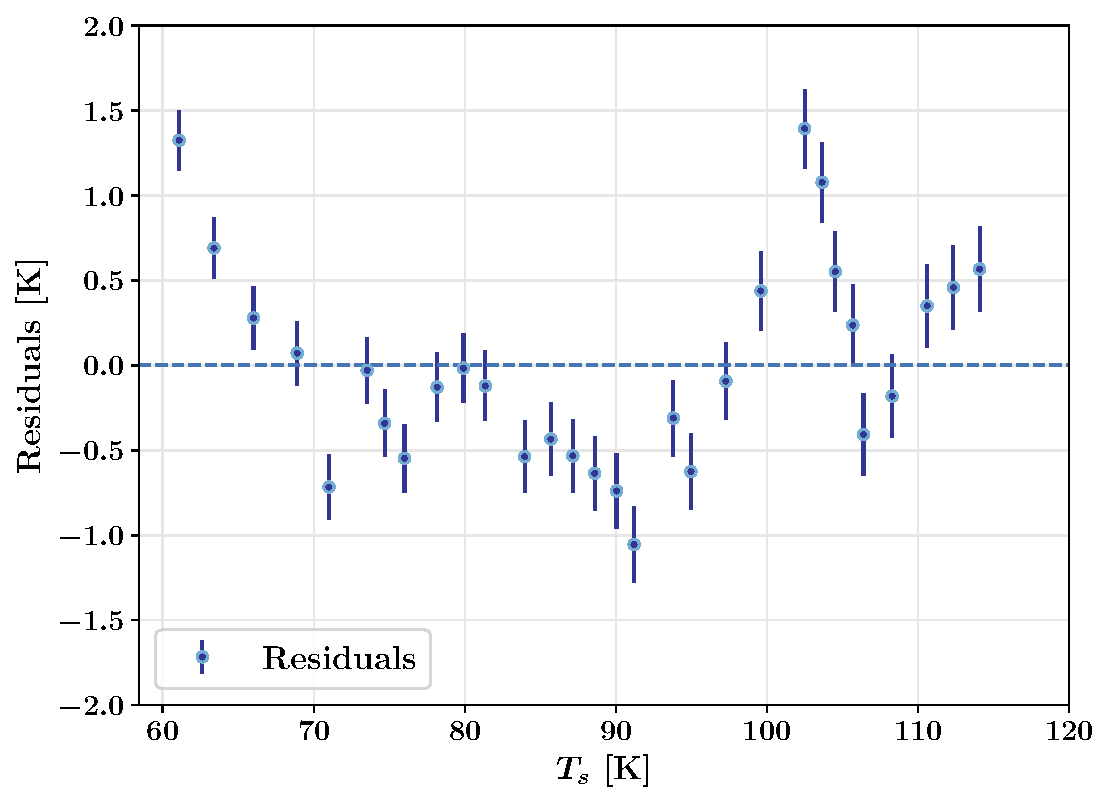
\includegraphics[width=\textwidth]{image/relation_plots/relation_res_co.pdf} \label{fig:res_cool_delay} }
\end{minipage}
\hfill
\begin{minipage}[]{0.49\linewidth}
\centering
\subfloat[Residuals of heating interpolation]{    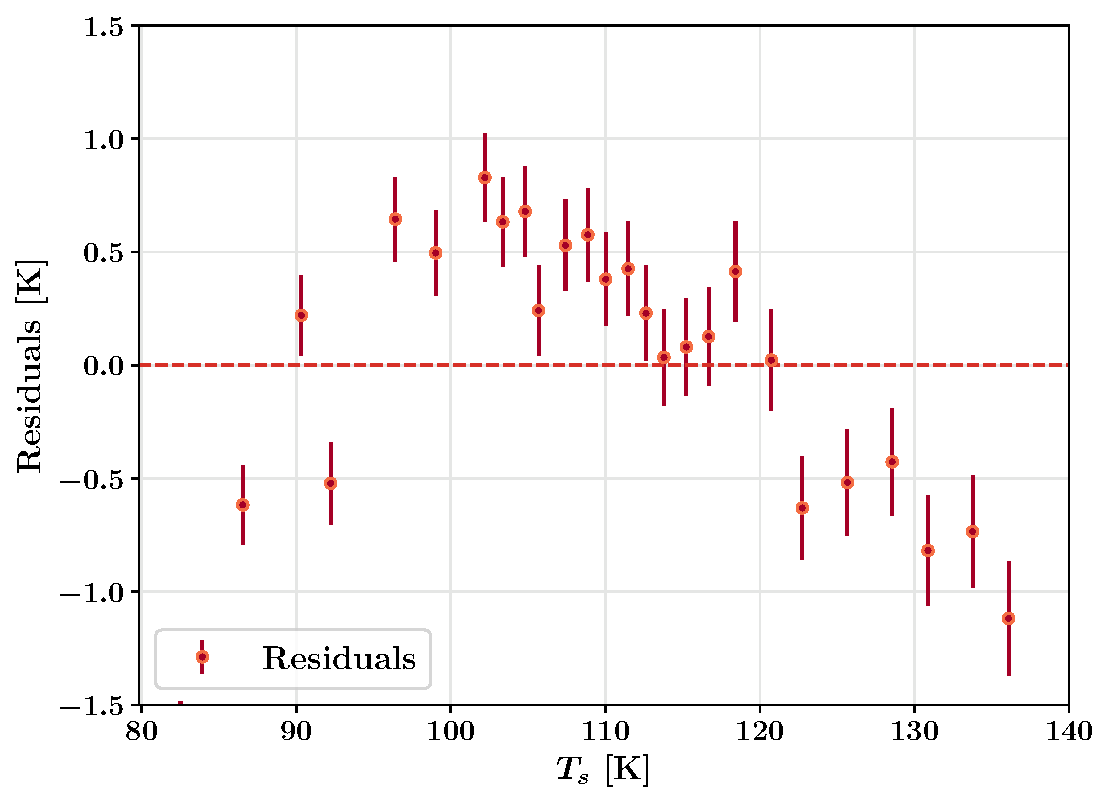
\includegraphics[width=\textwidth]{image/relation_plots/relation_res_he.pdf}\label{fig:res_hot_delay} }
\end{minipage}
\label{fig:delay_evaluation}
\caption{Relationship between the temperatures of the two platinum thermometers Pt100-cf and Pt100-s. In \ref{fig:res_cool_delay} and \ref{fig:res_hot_delay} are the residuals of the linear interpolations.}
\end{figure}

\pagebreak 

In both cases, the residuals placements around zero are not fully random but show a distinctive trend. This happens because the linear interpolation does not fully enclose the variability of the data, similarly to the fit of the background performed in SEC. \ref{subsubsec:drift_measurement}. Also in this case, we stick to the linear model for simplicity. Additionally, since the Pt100-s temperatures are collected manually, they are not taken exactly at the same instant as the Arduino ones. This contribution to the error, caused by the operator, is difficult to quantify and thus is ignored, despite the fact that this leads to an underestimation of the errors. Due to all these reasons, the values of $\chi^{(2)}$ to are quite big, about an order of magnitude greater than the expected value (leading also to almost null p-values). Nonetheless, the Pearson coefficients $r$ highlight a good level of linear correlation.

 \begin{table}[H]
    \sisetup{separate-uncertainty}
    \begin{tabular*}{\linewidth}{@{\extracolsep{\fill}}
    l 
    l 
    S[table-format=2.1(1)]  %intercept
    S[table-format=1.3(3)] %slope
    c 
    l 
    l 
    c
    c %S[table-format=3.1(1)]
    }
        \toprule
    & \textbf{Linear fit} & \textbf{Intercept [\si{\kelvin}]} &  \textbf{Slope} & $\pmb{r}$ & \textbf{$\pmb{\chi^{(2)}}$/ndf} & \textbf{p-value} & $\pmb{T_c^{\text{corr}}}$ \\
        \colrule
    {\color{cool}\textbf{Cooling}} & $\pmb{a_c + b_c \, x }$ &  48.4\pm0.2 & 0.731\pm0.003  & 0.9985 & 247.98/28 & 0 & \tablenum{107\pm1}\\
    \colrule
    {{\color{hot}\textbf{Heating}}} & $\pmb{a_h + b_h \, x }$ &  16.6\pm0.3 & 0.834\pm0.003 & 0.9987 & 262.60/24 & 0& \tablenum{107\pm3} \\
    \botrule
    \end{tabular*}
    \caption{Parameters of the linear fits performed on the $T_{cf}$ vs $T_{s}$ data. The Pearson coefficient $r$, $\chi^{(2)}$/ndf and right-tail p-value are also listed. The last column lists the Arduino estemates of $T_c$ corrected using the interpolating line}
    \label{tab:arduino_correction}
    \end{table}

The corrected estimates of $T_c^{corr}$ are now compatible within their experimental error with compatibility $\lambda = 0.009$ as the hysteresis has been counterbalanced. Given their compatibility, one can take as final estimate of the critical temperature the weighted average of the two $T_c$ from heating and cooling:
\begin{equation*}
    T_c^{Ard} = (107 \pm 1) \, \si{\kelvin}
\end{equation*}


\subsection{Manual equilibrium data}
\label{subsec:manual_equilibrium_data}

The experimental measurements taken with the temperature control procedure described in SEC. \ref{subsec:manual_equilibrium_acquisition} are illustrated in FIG. \ref{fig:equilibrium_data}. The errors on $\Delta V$ are obtained by propagation of random error on the difference $V_{out}-V_{off}$.

\begin{figure}[h!]
    \centering
    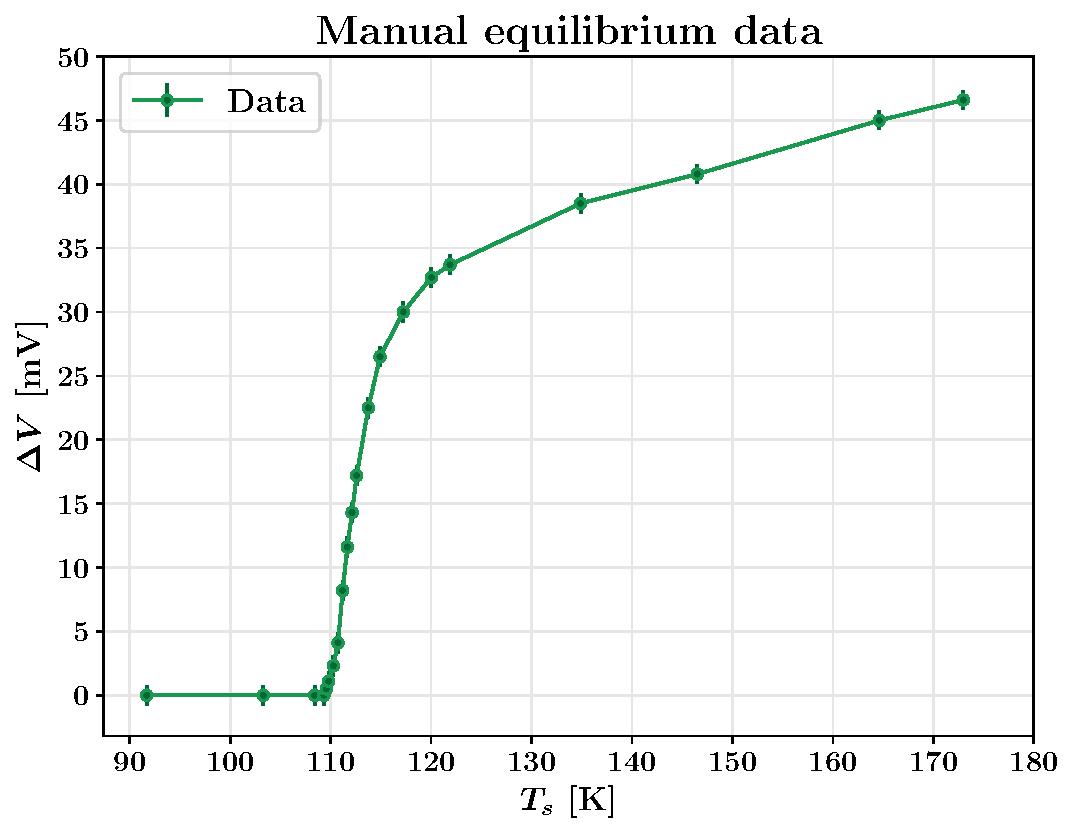
\includegraphics[width=0.7\textwidth]{image/equilibrium_plots/equilibrium_data.pdf}
    \caption{Voltage difference $\Delta V$ across the SC as a function of the temperature $T_s$ of the Pt100-s with temperature control. $\Delta V$ is the difference between the values of $V_{out}$ when $V_0 = \SI{6}{\volt}$ and $V_{off}$ when $V_0$ is turned off.}
    \label{fig:equilibrium_data}
\end{figure}

\pagebreak

The data immediately highlights how this procedure is much more accurate and reliable than the one previously followed. Thus, it is possible to carry out a more thorough analysis. For example, together with the critical temperature $T_c$, we can try to quantify range of temperatures $\Delta T_c$ over which the transition occurs. 

To begin with, a procedure similar to the ones described in the previous sections is carried out: we interpolate the transition region with a line $\Delta V = a_t + b_t \, T_s$ and estimate $T_c$ as the crossing of this line with the $x$ axis. The result is:
\begin{equation*}
    T_c^{eq} = (109.9 \pm 0.2) \, \si{\kelvin}
\end{equation*}

Then, the procedure schematized in FIG. \ref{fig:eq_proc} is followed. Firstly, a linear fit of the portion of the curve in the normal conductive region $\Delta V = a_n + b_n \, T_s$  is performed. Consequently, we consider also the three lines having respectively $10\%$, $50\%$ and $90\%$ of the height of this line. The transition range $\Delta T_c$ is defined as the range between the intersections of the transition region fit with the two lines at $10\%$ and $90\%$:
\begin{equation*}
    \Delta T_c = T_{c,0.9} - T_{c,0.1} 
\end{equation*}
where $T_{c,0.9}$ is the crossing with the $90\%$ line and $T_{c,0.1}$ the same but with the $10\%$ one.

Moreover, we can also evaluate the centroid of the transition range $\bar{T}_c$, temperature at the intersection of the transition line with the $50\%$ one.

The procedure described is commonly used as a standard method to derive $T_c$ for composite superconductors where the transition is less sharp \cite{metodo_tc}, \cite{HTC_springer}.

All the quantities related to the fits mentioned so far are listed in TAB. \ref{tab:equilibrium_coefficients} whereas the estimates of the various crossing points of interest are in TAB. \ref{tab:tc_result_equilibrium}. The error associated to these points is calculated as before (SEC. \ref{subsubsec:arduino_estimate_critical_temperature}).

\begin{table}[h!]
\centering
    \sisetup{separate-uncertainty}
    \begin{tabular*}{0.8\linewidth}{@{\extracolsep{\fill}}
    l 
    S[table-format=3(1)]  %intercept
    S[table-format=1.3(3)] %slope
    S[table-format=1.5]
    l 
    l 
    }
        \toprule
     \textbf{Linear fit} & \textbf{Intercept [K]}  & \textbf{Slope [K/$\pmb{\Omega}$]} & $\pmb{r}$ & \textbf{$\pmb{\chi^{(2)}}$/ndf} & \textbf{p-value} \\
        \colrule
     $\pmb{a_t + b_t \, x }$ & -221\pm19 & 2.0\pm0.2 & 0.994 & 1.59/5 & 0.902 \\
     $\pmb{a_n + b_n \, x }$ &  3\pm1 & 0.072\pm0.009 & 0.9994 & 0.0077/2 & 0.996 \\
    \botrule
    \end{tabular*}
    \caption{Parameters of the linear fit of the normal conductive region $(a_n + b_n T)$ and the transition region $(a_t + b_t T)$ with Pearson coefficient r, $\chi^{(2)}$/ndf and p-value.}
    \label{tab:equilibrium_coefficients}
\end{table}
    
\begin{table}[h!]
\centering
    \sisetup{separate-uncertainty}
    \begin{tabular*}{0.6\linewidth}{@{\extracolsep{\fill}}
    l 
    S[table-format=3(1)] 
    S[table-format=3.1(1)] 
    S[table-format=3.1(1)]
    c %S[table-format=3.1(1)]
    }
        \toprule
      & \textbf{90 \%}  & \textbf{50 \%} & \textbf{10 \%} & \textbf{y = 0}  \\
        \colrule
     $\pmb{T_c [K]}$ & 115 \pm 1 & 113 \pm 1 & 110 \pm 1 & \tablenum{109.9 \pm 0.2} \\
     $\pmb{R(T_c) [m \Omega]}$ & 10 \pm 2 & 5.5 \pm 0.9 & 1.1 \pm 0.2 & $-$ \\
    \botrule
    \end{tabular*}
    \caption{Critical temperature estimates for the different method for thermal equilibrium dataset.}
    \label{tab:tc_result_equilibrium}
\end{table}


As regards $a_t + b_t x$, the value of $\chi^{(2)}$ is of the same order of magnitude as its ndf, although a bit smaller. The residuals in FIG. \ref{fig:eq_res_trans} are dispersed around zero without a defined trend and are not too far from it.   
On the other hand for $a_n + b_n x$, the value of $\chi^{(2)}$/ndf is quite small because the errors are a bit overestimated with respect to the proximity of these experimental point to the theoretical curve. It is worth mentioning that in both cases the number of points fitted is quite limited thus making $\chi^{(2)}$ a not very meaningful indicator. Nonetheless, the Pearson coefficients $r$ highlight in all cases a good level of linear correlation in the data.

The results of this analysis are:
\begin{equation*}
    \Delta T_c = (5 \pm 2)\, \si{\kelvin}, \qquad  \bar{T}_c = (113 \pm 1) \, \si{\kelvin}
\end{equation*}

\pagebreak 

\begin{figure}[h!]
\begin{minipage}[c]{0.7\linewidth}
\subfloat[Estimation of $\Delta T_c$ and $\bar{T}_c$]{ 
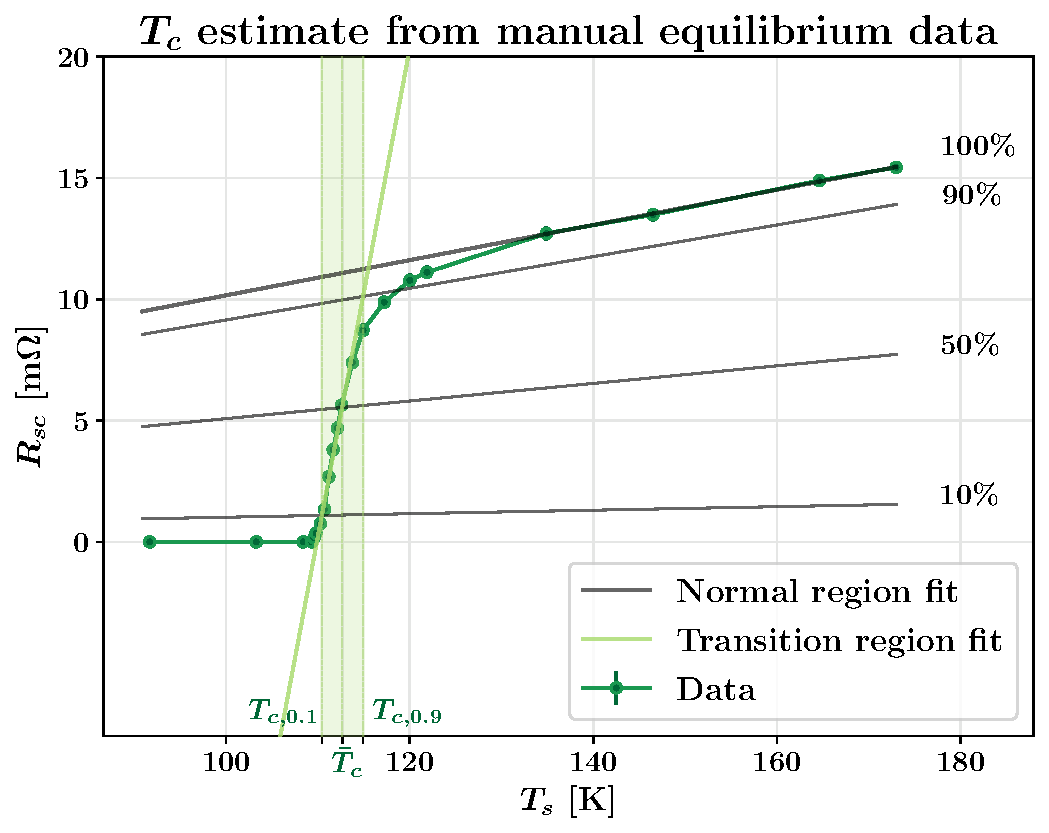
\includegraphics[width=\textwidth]{image/equilibrium_plots/equilibrium_tc.pdf} \label{fig:eq_proc} } 
\end{minipage} \\
\vspace{0.5cm}
\begin{minipage}[c]{0.49\linewidth}
\subfloat[Residuals of transition region interpolation]{  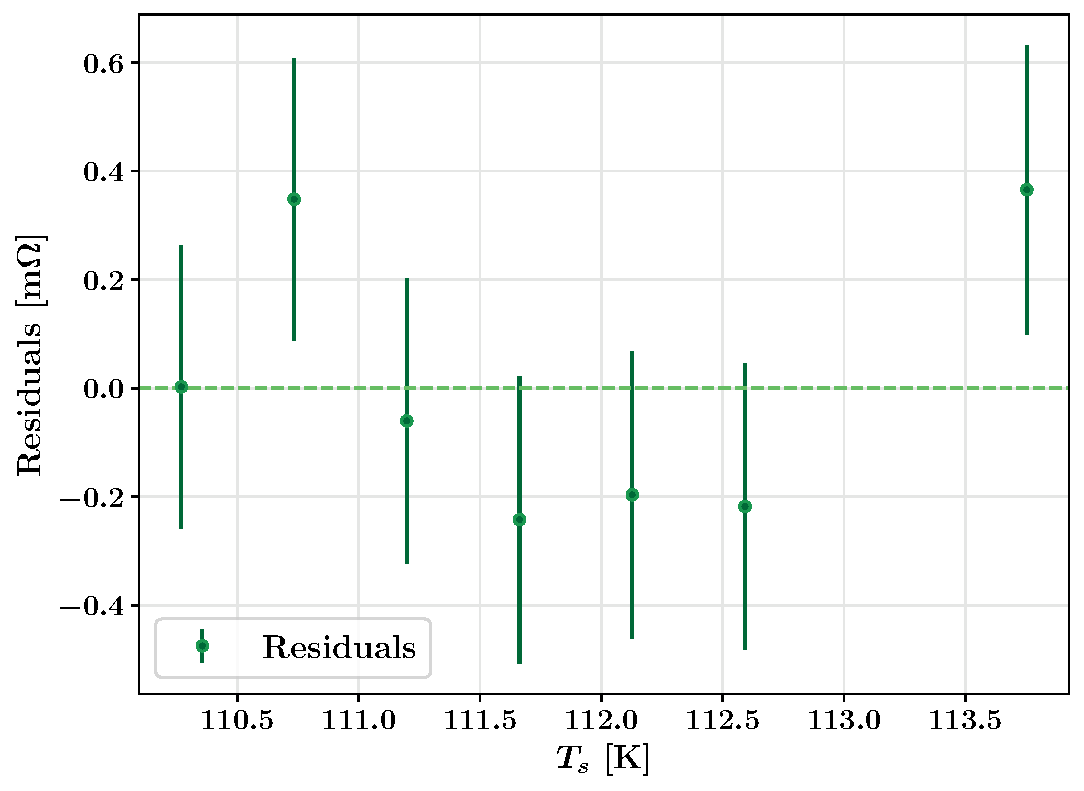
\includegraphics[width=\textwidth]{image/equilibrium_plots/equilibrium_transition_res.pdf} \label{fig:eq_res_trans} }
\end{minipage}
\hfill
\begin{minipage}[]{0.49\linewidth}
\centering
\subfloat[Residuals of normal region interpolation]{    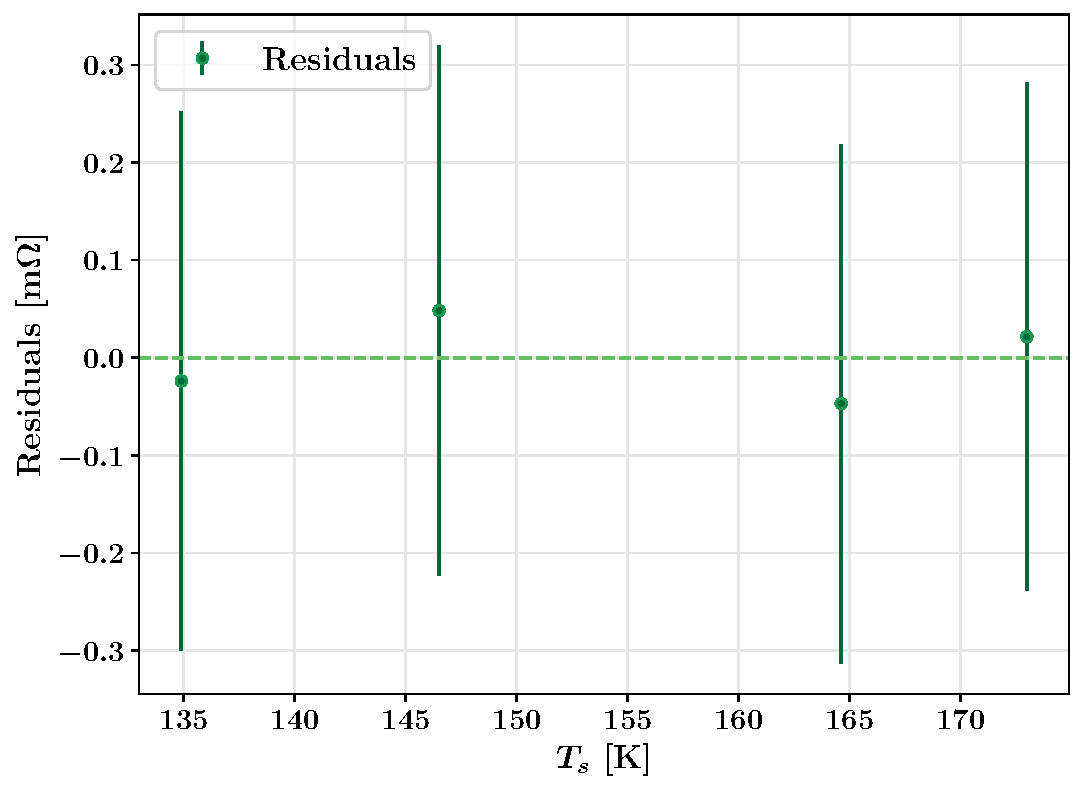
\includegraphics[width=\textwidth]{image/equilibrium_plots/equilibrium_normal_res.pdf}  \label{fig:eq_res_norm} }
\end{minipage}
\label{fig:equilibrium_estimate}
\caption{Estimate of the transition region $\Delta T_c$ and the centroid $\bar{T}_c$ from the Pt100-s with temperature control.
FIG. \ref{fig:eq_proc} depicts the procedure followed \cite{metodo_tc}, \cite{HTC_springer}. In FIG. \ref{fig:eq_res_norm} and \ref{fig:eq_res_trans} are the residuals of the fits in the normal conductive region and in the transition one.}
\end{figure}


 

\pagebreak

\section{Discussion}
\label{sec:discussion}

In this section the results obtained so far (summed up in TAB. \ref{tab:all_tc_estimates}) will be reviewed and compared. These values all suggest that our sample is most likely a bar of BSCCO-2223 with an expected critical temperature of about $\sim \SI{110}{\kelvin}$.

\begin{table}[h!]
\centering
    \sisetup{separate-uncertainty}
    \begin{tabular*}{0.6\linewidth}{@{\extracolsep{\fill}}
    l 
    c%S[table-format=3(1)] 
    c%S[table-format=3.1(1)] 
    c%S[table-format=3.1(1)]
    c%S[table-format=3.1(1)]
    }
        \toprule
      & \textbf{Cooling}  $\pmb{[K]}$ & \textbf{Heating} $\pmb{[K]}$ & \textbf{Final estimate} $\pmb{[K]}$\\
        \colrule
     \textbf{Arduino} & \tablenum{80 \pm 1} & \tablenum{109 \pm 3} & $-$  \\
     \textbf{Arduino corrected} & \tablenum{107 \pm 1} & \tablenum{107 \pm 3} & \tablenum{107 \pm 1}  \\
     \textbf{Manual drift} & \tablenum{106.4 \pm 0.4} & \tablenum{107.0 \pm 0.6} & \tablenum{106.8 \pm 0.2}  \\
     \textbf{Manual equilibrium} & $-$ & $-$ & \tablenum{109.9 \pm 0.2}  \\
    \botrule
    \end{tabular*}
    \caption{Summary of the critical temperature estimates from all the methods followed.}
    \label{tab:all_tc_estimates}
\end{table}

To begin with, it should be stressed that, even if in this report only the results for $V_0 = \SI{6}{\volt}$ are discussed, other values of input voltage for the amplifier circuit were tested. The choice of $V_0$ mostly affects the absolute value of $V_{out}$ and the entity of the voltage drop, but the temperature at which this drop occurs turns out to be consistent between the different values. The value $V_0 = \SI{6}{\volt}$ was chosen for the final estimates as it proved to be the best compromise between having an output high enough to be able to discern the jump from the background, but not too high as to avoid self-heating. As a matter of fact, using a too high value of $V_0$, would increase the power dissipated on the sample causing self-heating. This should cause discrepancies in the value of the transition temperature recorded by the Pt100-s between cooling and heating, similarly to what happens for the Arduino measurements with Pt100-cf. 

On the matter of the Arduino measurements, it can be seen that the limited resolution of the device has quite a strong impact on their quality. In fact, the voltage jump is just about 4 times bigger than the Arduino resolution, bringing to a quite poor SNR. Additionally, these estimates testify the importance of having a good thermal coupling between the sample and the thermometer: even having the Pt100-cf in a slightly different position with respect to the sample causes a big systematic error in the estimate of $T_c$. On the light of these results, we can say that the two values are mostly useful to detect the range of temperatures at which the transition occurs as they are inaccurate and imprecise. The only way to consider them to obtain an estimate of $T_c$  is to quantify the delay of the sample with respect to the cold finger as done in SEC. \ref{subsubsec:correction_arduino}. We can see that after of this procedure the hysteresis is corrected and the estimates become compatible with each other. 

The results from the manual drift analysis are more accurate and precise and the systematic error due to the bad thermal coupling is absent. However, it can be noticed that the final value is a bit lower than the one obtained with temperature control and the theoretical one. This discrepancy is most likely related to the influence of the range considered for the interpolation of the transition region. In this sense, the equilibrium measures are more reliable as they are already stripped from the background.
On the other hand, the results of the analysis in SEC. \ref{subsec:manual_drift_data} are strongly affected by the background subtraction procedure. We saw in fact that the trend of the underlying electromotive force is not constant and thus the boundaries of the transition region are strongly affected by the shape assumed for the background.

All these considerations lead us to pick the manual equilibrium measure as best estimate of the critical temperature of the superconductor sample.
The equilibrium measures also allow us to determine the range of transition. High-temperature superconductors are characterized by a transition which is not too sharp and for this reason some might consider $T_c$ as the centroid of this transition regime. Following the method described in SEC. \ref{subsec:manual_equilibrium_data} the transition is determined to be centered around $\bar{T}_c = (113 \pm 1)\, \si{\kelvin}$ with a range $\Delta T_c = (5\pm 2)\, \si{\kelvin}$.

\section{Conclusions}
\label{sec:conclusions}
The results suggest that the composition of the cuprate high-temperature superconductor analysed is mostly BSCCO-2223. 
The best estimate of its critical temperature, taken as $T$ at which the resistivity becomes exactly zero, is $T_c = (109.9 \pm 0.2)\, \si{\kelvin}$.
Moreover, the transition is centered around $\bar{T}_c = (113 \pm 1)\, \si{\kelvin}$ and spreads over a range of $\Delta T_c = (5\pm 2)\, \si{\kelvin}$.

\clearpage

\bibliographystyle{plain}

\bibliography{references}{}

\end{document}
